%!TEX root = ../thesis.tex
%*******************************************************************************
%****************************** Third Chapter **********************************
%*******************************************************************************
\chapter{The Short-Baseline Near Detector and The Booster Neutrino Beam}

% **************************** Define Graphics Path **************************
\ifpdf
    \graphicspath{{Chapter4/Figs/Raster/}{Chapter4/Figs/PDF/}{Chapter4/Figs/}}
\else
    \graphicspath{{Chapter4/Figs/Vector/}{Chapter4/Figs/}}
\fi

%********************************** %Opening  **************************************

The Short-Baseline Near Detector is an integral part of the Short-Baseline Neutrino program at Fermilab, designed to investigate sterile neutrino-induced oscillations. 
The proposal is driven by anomalous results observed across various detectors involving accelerator, nuclear reactor, and solar neutrino experiments.
SBND also has its own extensive program focusing on neutrino cross-section and beyond the Standard Model physics. 
This will not only benefit future neutrino experiments such as DUNE but also significantly advance the field of neutrino physics.
As of 2024, SBND has entered its commissioning phase, preparing for calibration and physics data taking.

This chapter begins with a discussion on the physics program of the SBND experiment in Sec. \ref{sec4PhysicsProgram}. 
Moreover, Sec. \ref{sec4SBND} provides a detailed description of SBND's detection hardware, covering the time projection chamber, photon detection system, and cosmic ray tagger system. 
This section also elaborates on the hardware triggering system and the data acquisition system employed at SBND.
Finally, an overview of the Booster Neutrino Beam (BNB) is presented in Sec. \ref{sec4BNB}, detailing the neutrino production process of the beam and provides insights into the flux prediction at SBND.

\newpage
%********************************** %First Section  **************************************
\section{The Short-Baseline Near Detector Physics Program}
\label{sec4PhysicsProgram}
%SBN Program

%0: SBND, as part of the SBN Program
%Neutrino Oscillation
The Short-Baseline Near Detector (SBND) is part of the Short-Baseline Neutrino (SBN) Program located at Fermilab \cite{SBNProgram}. 
The program consists of three LArTPC detectors: SBND, MicroBooNE, and Imaging Cosmic Rare Underground Signals (ICARUS), positioned at distances of 110 m, 470 m, and 600 m, respectively, on axis to the target of the Booster Neutrino Beam (BNB) as shown in Fig. \ref{fig:SBN_program}.
The near-far detector setup was designed to search for the potential existence of sterile neutrinos with an eV mass scale, driven by a series of anomalies observed by previous short baseline experiments.

The Liquid Scintillator Neutrino Detector (LSND) experiment utilised a stopped pion source to probe $\bar{\nu}_{e}$ via inverse beta decay and reported an excess of signal to background at low energies with a 3.8$\sigma$ level \cite{LSND_anomaly}. 
Meanwhile, the MiniBooNE experiment was a neutrino accelerator experiment to measure the entire phase space covered by the LSND result \cite{Miniboone_anomaly}.
The detector observed an excess of $\nu_{e}$ ($\bar{\nu}_{e}$) in $\nu_{\mu}$ ($\bar{\nu}_{\mu}$) beam mode showing a discrepancy from the SM with a significance level of 4.5$\sigma$ (2.8$\sigma$), reaching 6.0$\sigma$ when combined with the LSND data.
Additionally, results from the nuclear reactor experiments indicated a deficit of $\bar{\nu}_{e}$ fluxes to expectations at a 3$\sigma$ level \cite{reactor_anomaly_1, reactor_anomaly_2}, as well contained spectral features consistent with a fourth neutrino addition \cite{reactor_anomaly_3, reactor_anomaly_4}.
Furthermore, gallium solar neutrino experiments observed an overall deficit in $\nu_{e}$ fluxes at a 3$\sigma$ level during calibrations using radioactive neutrino sources \cite{galium_anomaly_1, galium_anomaly_2}.
These four main anomalous results collectively suggest the mixing of SM neutrinos with a fourth non-weakly-interacting neutrino at a short baseline to energy ratio of $L/E \approx 1 $ m/MeV, a phenomenon known as sterile neutrino oscillation \cite{SBNProgram}.
The goal of the SBN program is to pioneer the search for eV-scale sterile neutrino oscillations,  covering the parameter phase space previously allowed by past experiments at a significance level of $\geq 5 \sigma$.

\begin{figure}[htbp] 
\centering    
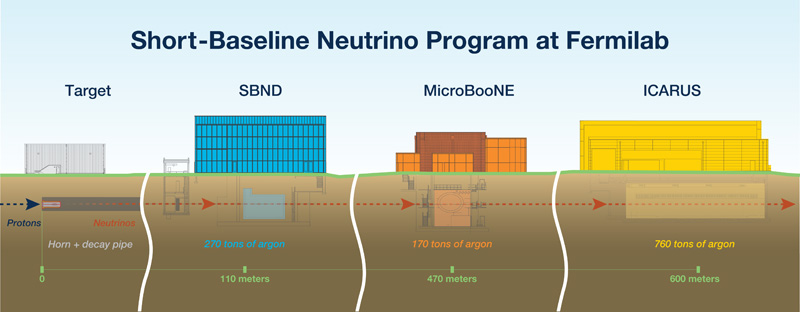
\includegraphics[width=1.0\textwidth]{SBN_program}
\caption[SBN_program]{
Graphic showing the three LArTPC detectors made up the Short-Baseline Neutrino program: SBND, MicroBooNE and ICARUS.
Their respective masses and distances with respect to the target of the Booster Neutrino Beam are shown.
Fig. from \cite{SBNProgram}.
}
\label{fig:SBN_program}
\end{figure}

%Neutrino Cross Section
Additionally, measurements of neutrino-nucleus interactions plays a crucial role in the physics program of SBND, serving as a critical element in understanding neutrino oscillation \cite{NuSTECWhitePaper}. 
Being the nearest to the beam, SBND is presented with a unique opportunity to observe the largest unoscillated neutrino fluxes among the three detectors.
Over the 3-year operational span, SBND aims to record a staggering 10 million neutrino events, originating from $10 \times 10^{20}$ Proton-On-Target (POT) interactions \cite{SBNProgram}.
This will establish SBND as the world leader in statistics for neutrino-argon cross section measurements.
More than 6 millions $\nu_{\mu}$ charged current (CC) events will be collected, reducing the statistics uncertainty well below the percent.
Moreover, SBND is expected to record 45,000 $\nu_{e}$ CC events, marking the most extensive statistics for both inclusive and exclusive measurements of this channel to date.
These measurements will be extremely beneficial for advancing the objectives of the SBN physics program, as well as contributing to the physics goals of the Deep Underground Neutrino Experiment (DUNE), which employs argon as its target material.

%BSM
Finally, a key aspect of the physics program of the SBND experiment is the exploration of new scenarios leading to BSM physics. 
Close proximity to a high-intensity beam and the resulting large statistics enable searches for very weakly coupled interactions coming from the BNB \cite{SBNProgram}.
%HNL
Namely, heavy neutral leptons, the primary focus of this thesis, can be produced by the BNB and subsequently decay in-flight into SM observables for detection \cite{SBNHNL}.
%Light Dark Matter
Another compelling BSM candidate is light dark matter, which can be produced from neutral meson decay or proton bremsstrahlung in the BNB \cite{LightDarkMatter}. 
Postulated by thermal relic models, these light dark matter particles could reach sub-GeV-scale masses. 
The particles may scatter and decay, resulting in electromagnetic showers without any hadronic activities inside the detector.
%Dark neutrino
Moreover, the dynamic mass mechanism of neutrinos opens avenues for new physics in the dark sector. 
The dark neutrino model proposes that right-handed neutrinos can scatter with nuclei to produce dark gauge bosons, subsequently decaying into di-lepton pairs \cite{DarkNeutrino}. 
In the case where the leptons are electrons, this could potentially explain the low energy excess anomalies observed by LSND and MiniBooNE \cite{DarkNeutrinoLEE}.
These represent just a few examples of the diverse array of BSM scenarios that can be explored at the SBND detector. 
Other unmentioned possibilities such as new interactions, extra dimensions, violations of Lorentz and CPT symmetries, among others, contribute to the rich physics program of SBND \cite{SBNProgram}.

%********************************** %First Section  **************************************
\section{The Short-Baseline Near Detector}
\label{sec4SBND}

The SBND detector is a LArTPC with an active volume of 112 tons and dimensions of 4 m (x-drift) $\times$ 4 m (y-height) $\times$ 5 m (z-length) \cite{SBNProposal}.
As depicted in Fig. \ref{fig:SBND_Pretty}, the detector consists of two separate TPCs, each with a drift length of 2 m, sharing a common Cathode Plane Assembly (CPA) positioned at the centre.
A sophisticated Photon Detection System (PDS) is located behind each Anode Plane Assembly (APA) at the edge of the detector.
Additionally, the PDS incorporates a passive component consisting of TPB-coated reflective foils installed at the CPA.
The entire detector is placed inside a membrane cryostat, and then is surrounded by seven planes of Cosmic Ray Tagger (CRT) modules to provide a full solid angle coverage for cosmic rejection.

\begin{figure}[htbp] 
\centering    
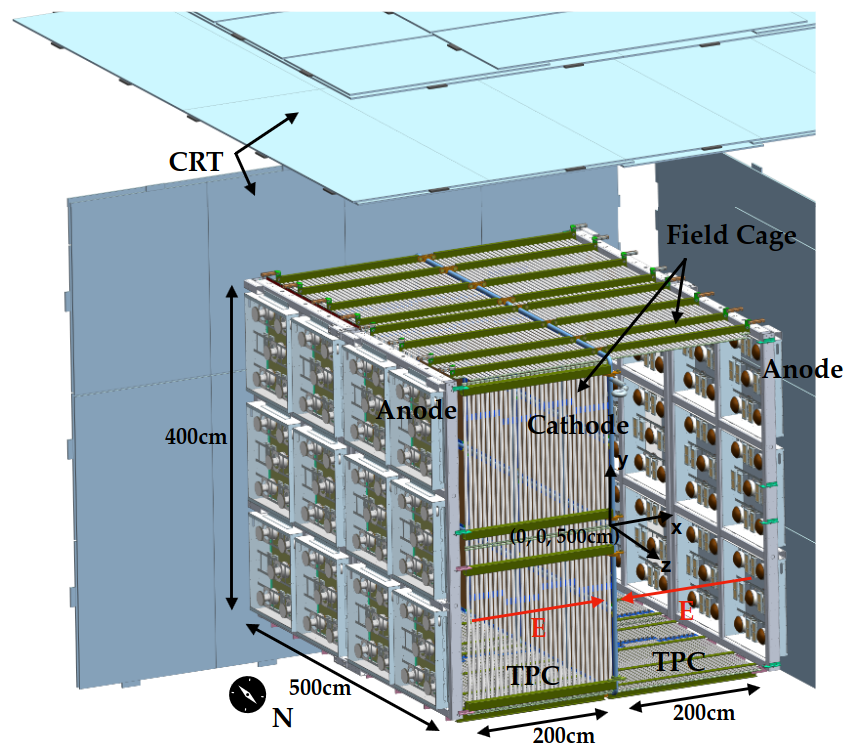
\includegraphics[width=0.70\textwidth]{SBND_Pretty}
\caption[SBND_Pretty]{
3D modelling of the SBND detector, showing the main LArTPC surrounded by 7 CRT planes.
The central CPA divides the detector into two TPCs, each with their own APA and PDS located behind the wire planes.
}
\label{fig:SBND_Pretty}
\end{figure}

\subsection{Time Projection Chamber}

The APA planes of the SBND TPC are illustrated in Fig. \ref{fig:SBND_APA}. 
A single APA measures 4 m $\times$ 2.5 m and comprises a steel frame supporting three wire planes: two induction planes, denoted as U and V, oriented at angles of $\pm 60^{\circ}$ to the vertical collection plane, denoted as Y. 
These wire planes U,V and Y are colour-coded as green, blue, and red, respectively.
Each wire plane is constructed with 150 $\mu$m diameter copper-beryllium wires, with a wire pitch and plane spacing of 3 mm. 
The wires are tensioned to 7 N to prevent slackening when cooled down to liquid argon temperature at 89 K \cite{SBND_Wires}.
To maintain charge transparency for the induction planes and collection efficiency for the collection plane, a biased voltage of -200 V, 0 V, and 500 V is applied to planes U, V, and Y, respectively.
A pair of coupled APAs together form an APA plane, utilizing jumper cables to bridge the 15 mm gap between the induction planes to form a single electronic channel. 
In total, each TPC consists of 5,632 wires: 1,664 wires in the collection plane and 1,986 wires in each induction plane.

\begin{figure}[hbp] 
\centering    
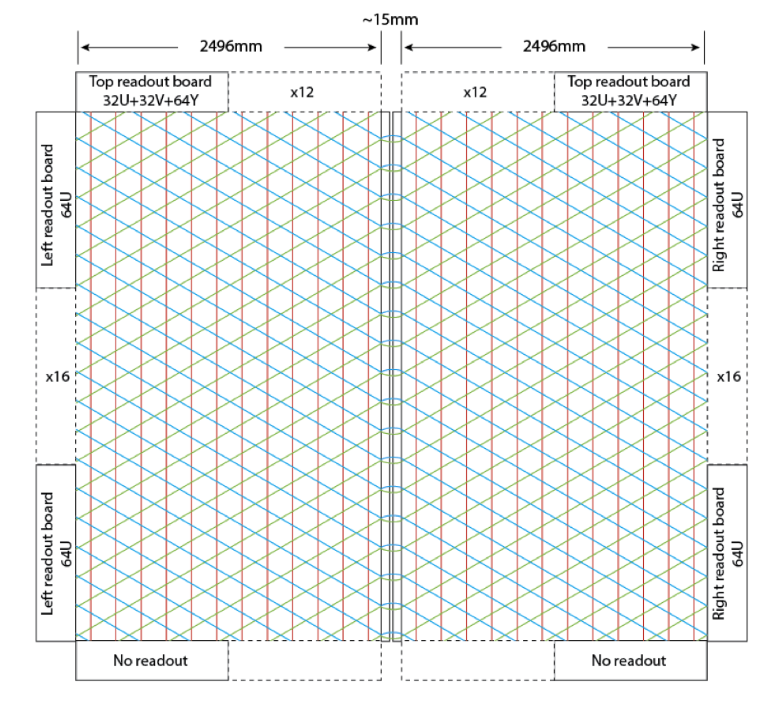
\includegraphics[width=0.70\textwidth]{SBND_APA}
\caption[SBND_APA]{
A schematic diagram showing two coupled APAs to form a single APA Plane.
The three wire planes U, V, Y are in colour green, blue and red respectively, along side the cold electronic readouts.
The induction planes of the APAs are coupled together across the 15 mm gap at the centre.
Fig. from \cite{SBNProposal}.
}
\label{fig:SBND_APA}
\end{figure}

%CPA
The CPA plane consists of two steel frames, each containing 8 windows, as illustrated in Fig. \ref{fig:SBND_CPA_APA}. 
Each window, measuring 60 cm $\times$ 50 cm, houses a fiberglass plate laminated on both sides with non-conductive reflective foils $> 99\%$ specular reflection in the visible range and coated with TPB.
Furthermore, the plate is covered by a wire mesh, which provides a biased voltage of -100 kV supplied by a high-voltage feedthrough donut from outside the cryostat.

%Field Cage
The field cage consists of a sequence of electrodes arranged perpendicular to the drift direction. 
These electrodes incrementally step up the voltage from -100 kV applied at the CPA to the ground voltage in increments of 3 kV. 
This gradual voltage increase is implemented to maintain a uniform electric field of 500 V/cm across the drift volume.

\begin{figure}[htbp!]
%\hfill
\begin{subfigure}[h]{0.5\linewidth}
\centering    
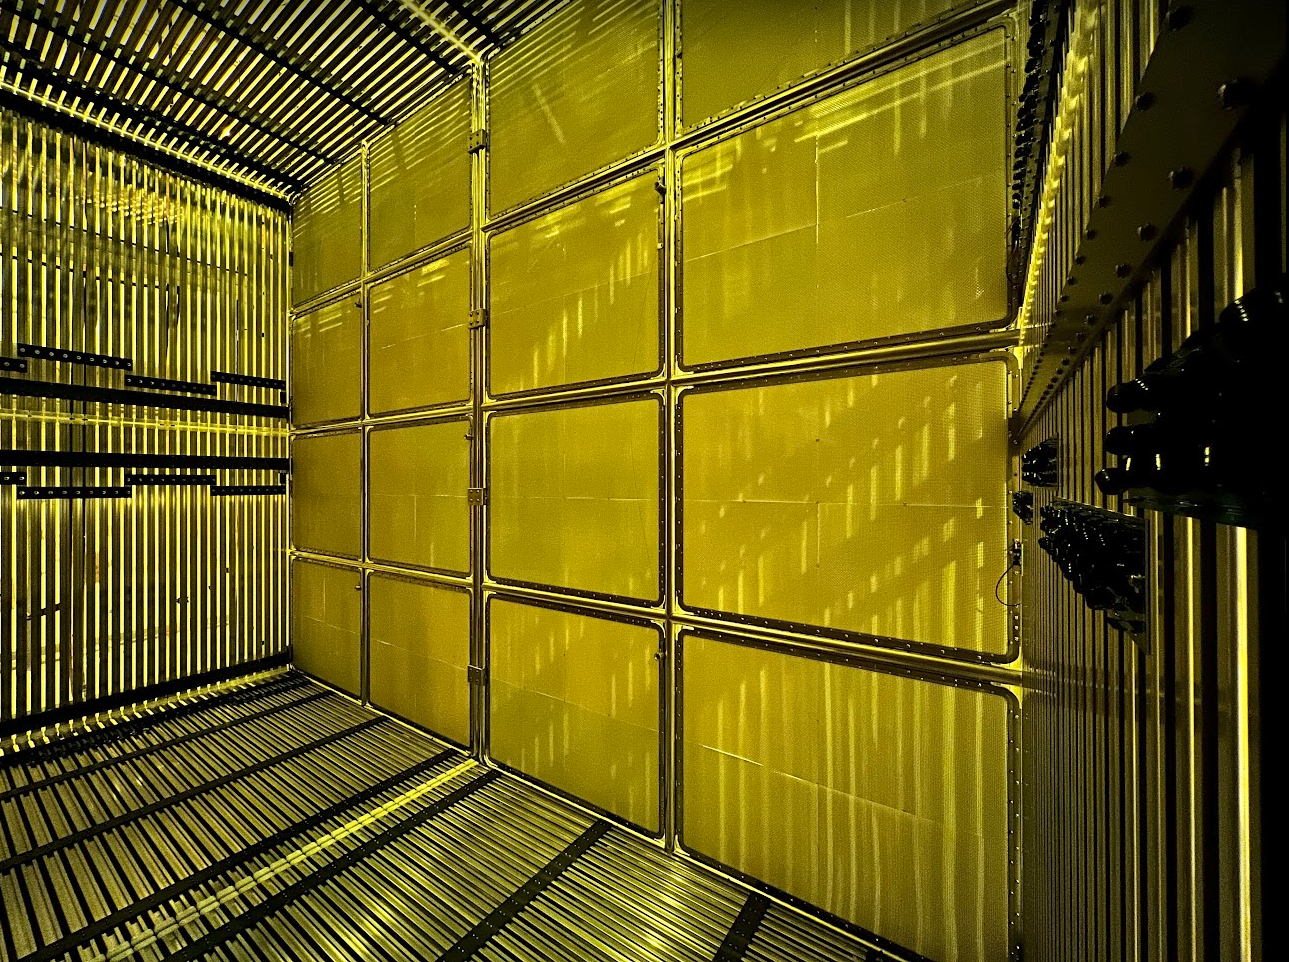
\includegraphics[width=\linewidth]{SBND_CPA}
\caption{View of the CPA}
\end{subfigure}
\hfill
\begin{subfigure}[h]{0.5\linewidth}
\centering    
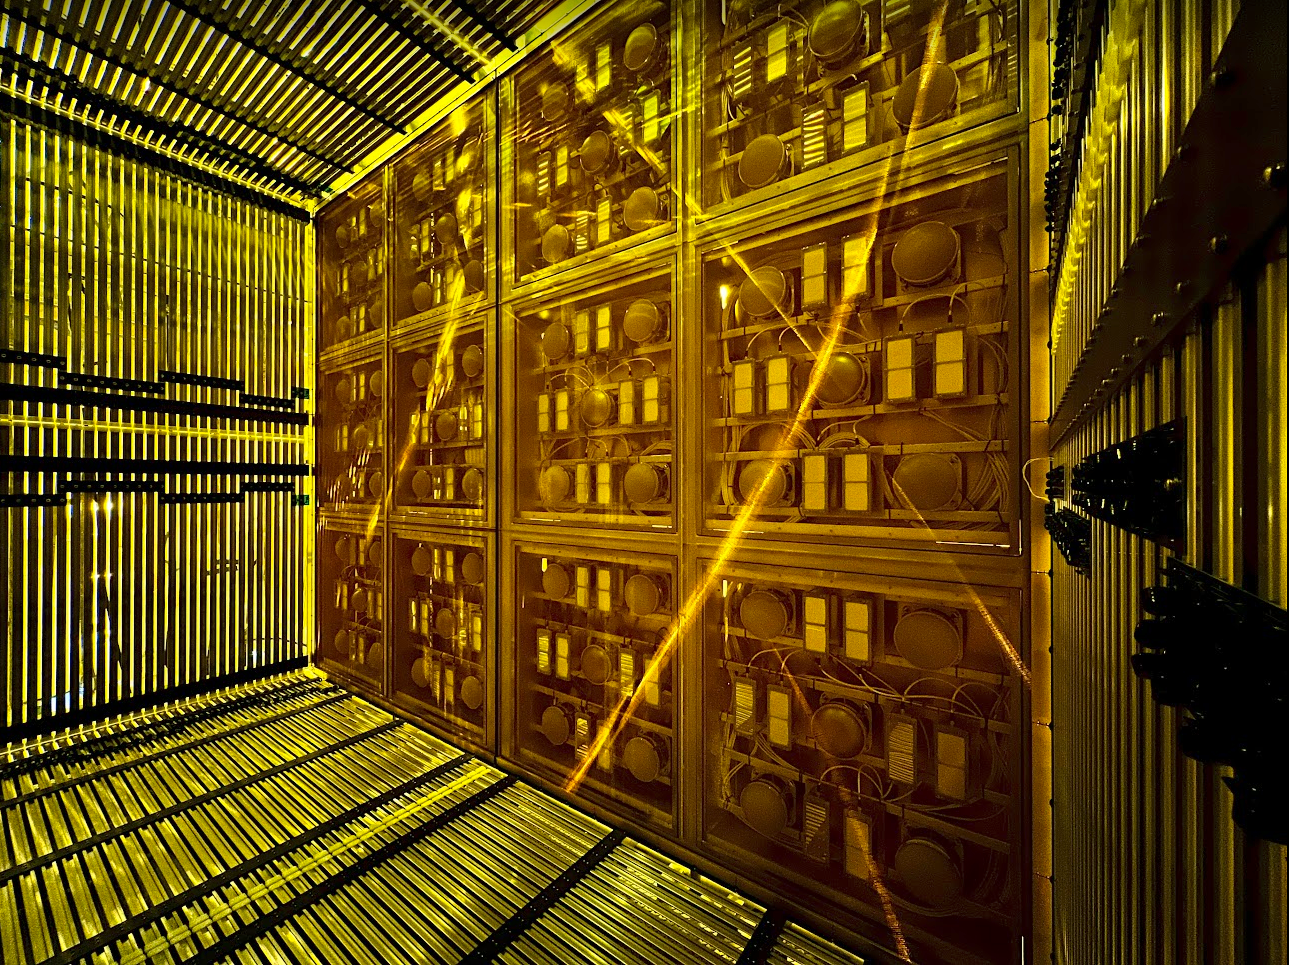
\includegraphics[width=\linewidth]{SBND_APA_PDS}
\caption{View of the APA}
\end{subfigure}%
%\hfill
\caption[SBND_CPA_APA]{
Photographs of the SBND detector during the construction phase at Fermilab. 
The left photo shows the central CPA housing 16 reflective foils coated with TPB.
The right photo shows the APA with the PDS located behind the wires.
The field cage can also be seen a series of metal bars surrounding the TPC.
}\label{fig:SBND_CPA_APA}
\end{figure}

\subsection{Photon Detection System}

%TODO: Add citation
%describe PMT, XARAPUCA and TPB
The design of the SBND Photon Detection System (PDS), incorporating both active and passive optical components, is the most sophisticated system ever installed in a LArTPC. 
The active detector integrates two different technologies: (1) a system of 120 Photomultiplier Tubes (PMTs) and (2) a system of 192 X-ARAPUCA devices.
The PMTs utilized are cryogenic 8"-diameter Hamamatsu R5912-MOD models \cite{hamamatsu}. 
Meanwhile, the X-ARAPUCAs serve as a research and development platform for future experiments, incorporating multiple variations in their components for performance comparison. 
A summary of the X-ARAPUCA specifications can be found in Ref. \cite{}.
The TPB-coated reflective foils installed at the CPA is the passive component of the PDS in order to achieve a uniform light yielf.

In SBND, the PMT system is the primary light detection system and is utilized to provide trigger conditions. 
The 120 PMTs are partitioned into two optically-isolated TPC volumes, each with 60 PMTs.
Within each TPC, 48 PMTs are TPB-coated, and thus are sensitive to both direct and reflected light components, while the remaining 12 non-coated PMTs detect only reflected light. 
This ratio of coated to uncoated PMTs (4:1) is chosen to optimize light collection efficiency while maintaining the capability to distinguish between the two light components. 
Such differentiation improves the reconstruction of scintillation light, which will be discussed in Sec. \ref{}.

%PDS Box
For the purpose of installation, the optical detectors are arranged into modular PDS boxes, as depicted on the left side of Fig. \ref{fig:SBND_PDS}. 
Each box houses 5 PMTs, 4 coated and 1 uncoated PMT, along with 8 X-ARAPUCA devices, 4 coated and 4 uncoated.
These PDS-boxes are installed in a configuration of $4 \times 3$ behind each APA plane, resulting in a total of 12 boxes per TPC volume, as illustrated on the right side of Fig. \ref{fig:SBND_PDS}.

\begin{figure}[hbp]
\centering    
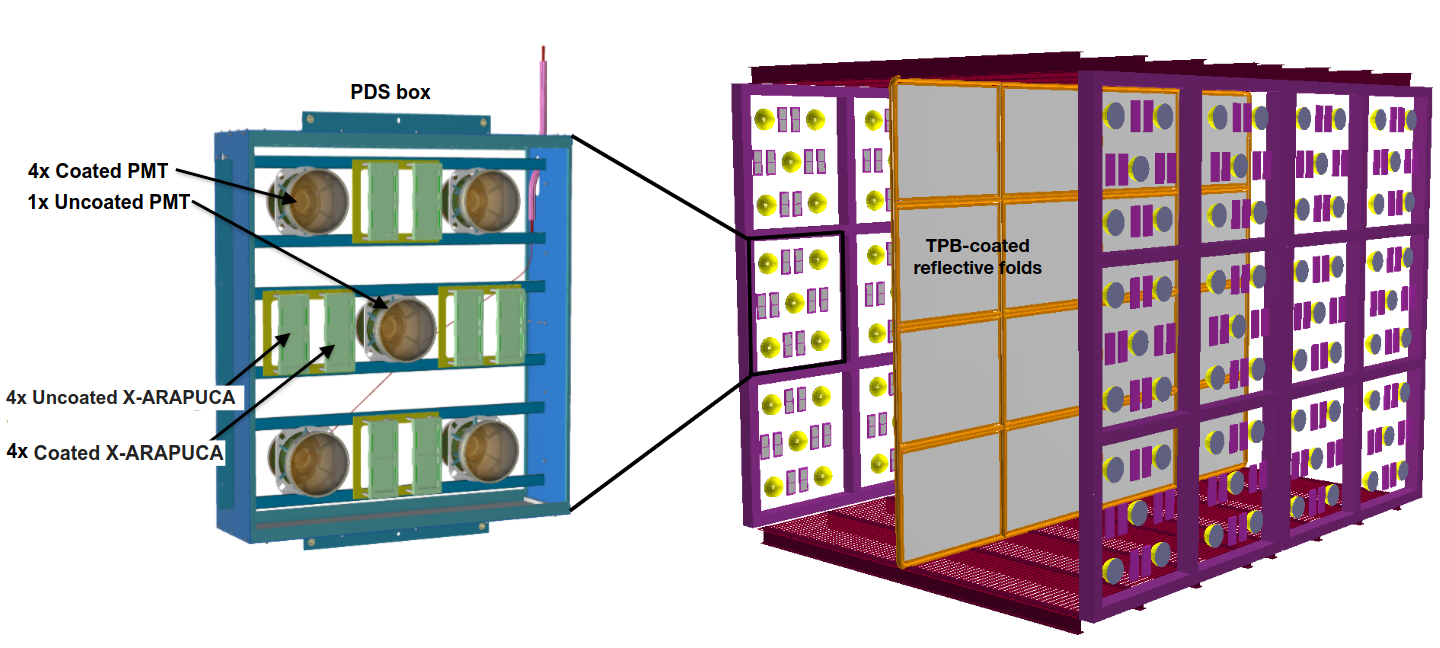
\includegraphics[width=0.95\textwidth]{SBND_PDS}
\caption[SBND_PDS]{
3D modelling of the PMTs and X-ARAPUCAs arrangement in a PDS box (left), together with the PDS boxes installation inside the TPC.
Fig. from \cite{}.
}
\label{fig:SBND_PDS}
\end{figure}

\subsection{Cosmic Ray Taggers}

Since SBND is a surface detector, it utilizes a Cosmic Ray Tagger (CRT) system to effectively reject background from cosmic rays. 
Each CRT strip consists of a plastic scintillator strip  with width of 10.8 cm, connected to a pair of SiPMs via wavelength-shifting optical fibres.
These CRT strips are arranged perpendicular to each other to construct a single CRT plane, as depicted in Fig. \ref{fig:SBND_CRT}, measuring 7.5 m in height and 9 m in width. 
Coincident hits from perpendicular strips allow for the 2D reconstruction of the hit location, and the number of photons collected for each strip improves the precision of the location tagging.
Signals from the SiPMs are amplified, digitized and readout by the Front End Board (FEB) modules with nanosecond timing resolution, which will be detailed in Sec. \ref{}.

As illustrated in Fig. \ref{fig:SBND_Pretty}, SBND is entirely encased by 7 CRT planes, with 1 on each side and 2 positioned atop the detector. 
This configuration enables a comprehensive strategy for cosmic background rejection utilising both geometrical and high-precision timing information.
For instance, tracks identified by the TPC can be matched to CRT hits to identify tracks occurring outside the beam spill window.
Additionally, the top 2 planes function as a telescopic array, facilitating the tagging of vertical downward-going cosmic rays.

\begin{figure}[htbp] 
\centering    
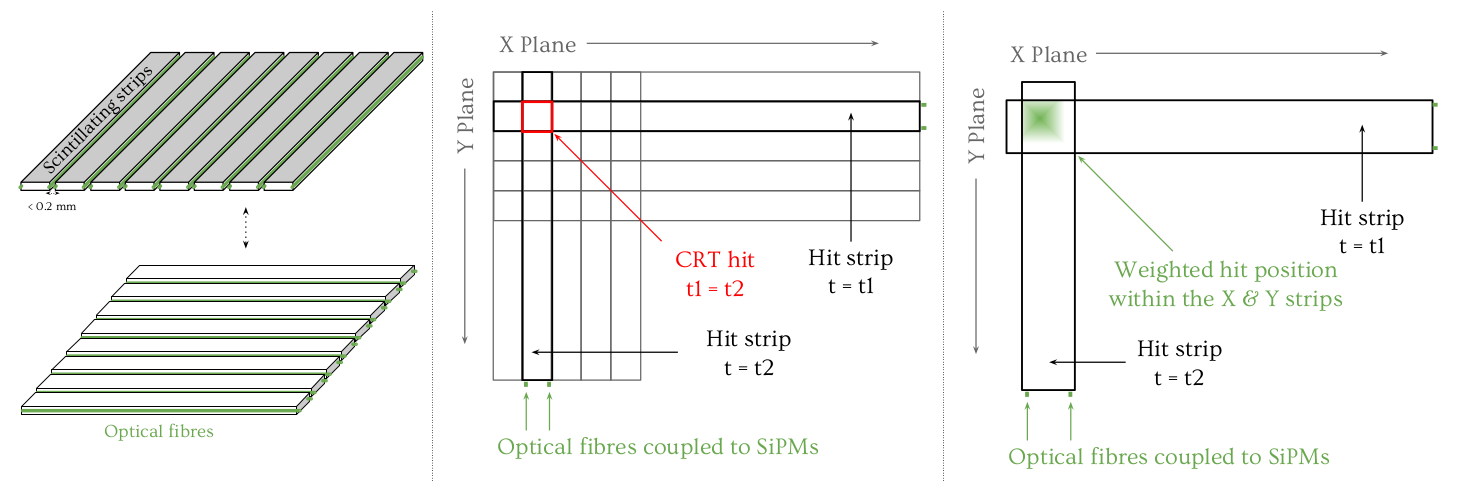
\includegraphics[width=1.0\textwidth]{SBND_CRT}
\caption[SBND_CRT]{
Each CRT plane contains 16 scintillating strips oriented orthogonal to each other (left).
Hits coincident in time from perpendicular strips can be used to tag the hit location (middle).
The number of photons collected by each hit improves the precision of location tagging (right).
Fig. from \cite{RhiannonPhD}.
}
\label{fig:SBND_CRT}
\end{figure}

\subsection{Trigger}

Triggering plays a vital role in the SBND detector, given its close proximity to the BNB and exposure to cosmic rays as a surface detector, resulting in a high rate events. 
The hardware trigger in SBND is issued by the Penn Trigger Board (PTB) \cite{ptb_gvs}, photographed in Fig. \ref{fig:SBND_PTB_MTCA}, which receives inputs from the beam system and two detection systems equipped with high timing resolution: the PMTs and CRTs. 
Notably, SBND marks the first instance of a LArTPC employing the CRT system as part of its triggering mechanism \cite{CPAD2022}.
The PTB then applies programmable trigger logic on the inputs to form triggers.
There are three primary types of triggers: (1) the beam trigger for acquiring physics data, (2) the off-beam trigger for estimating cosmic background, and (3) the calibration trigger.

\begin{figure}[tbp!]
%\hfill
\begin{subfigure}[h]{0.5\linewidth}
\centering    
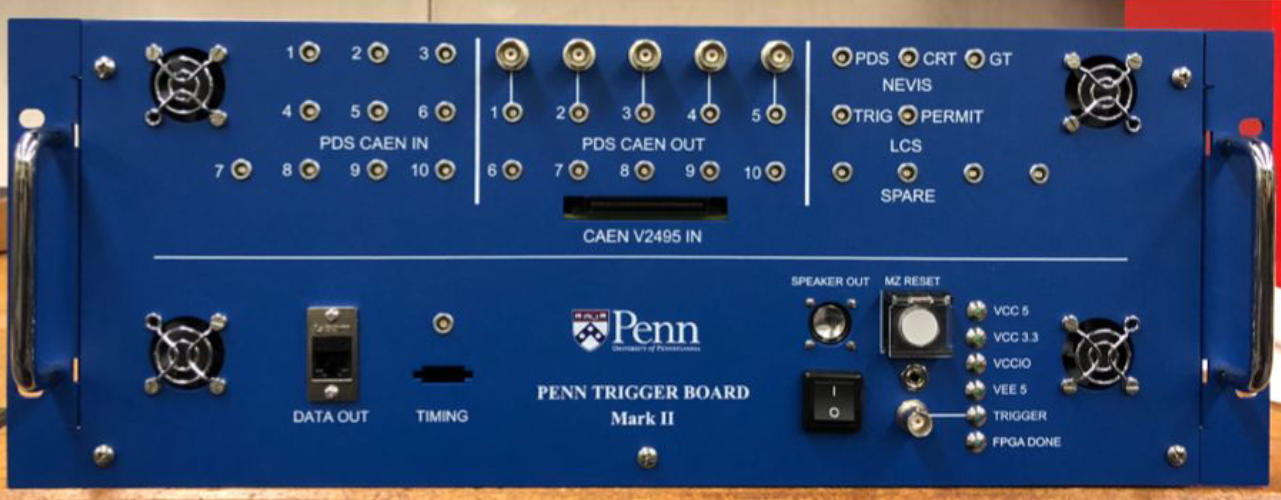
\includegraphics[width=\linewidth]{SBND_PTB}
\caption{Penn Trigger Board}
\end{subfigure}
\hfill
\begin{subfigure}[h]{0.5\linewidth}
\centering    
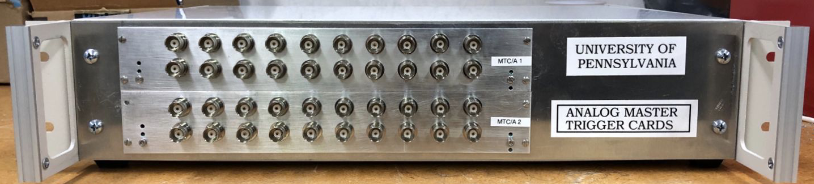
\includegraphics[width=\linewidth]{SBND_MTCA}
\caption{Master Trigger Card Analog}
\end{subfigure}%
%\hfill
\caption[SBND_PTB_MTCA]{
Photographs of the two hardware components in the SBND triggering system.
}\label{fig:SBND_PTB_MTCA}
\end{figure}

Diagram in Fig. \ref{fig:SBND_Trigger} depicts the signal inputs and outputs to and from the PTB to detection subsystems.
The beam system informs the PTB about the status of the BNB beam, indicating whether the beam has arrived at the detector hall (shown in green).
The PMTs provide information regarding the energy deposited inside the detector (shown in light blue).
The number of PMT pairs above a predefined threshold, known as PMT multiplicity, is calculated by the Master Trigger Card Analog (MTC/A) to provide information of the PMT locations (shown in red).
The primary beam trigger requires the PMT multiplicity to coincide with the beam window. 
Conversely, for background estimation purposes, anti-coincidence logic can be applied to estimate the cosmic rate.
Meanwhile, the CRT system provides versatile information regarding the topology of cosmic tracks (shown in purple). 
The calibration trigger utilises the CRTs in coincidence with the PMTs to select cosmic tracks of specific topologies. 
For example, anode-to-cathode-crossing cosmic tracks can be employed for electron lifetime measurements, which will be explored in Sec. \ref{}.

Once a trigger is formed, the PTB send the signals to subsequent readout subsystems to acquire the event (shown in pink).
An event contains two types of trigger signals: a single Event Trigger (ETRIG) and multiple Flash Triggers (FTRIGs).
The ETRIG is issued to the TPC readouts to acquire waveforms from the wire planes. 
Conversely, FTRIGs are issued to the PDS readouts to capture waveforms from the optical detectors. 
Further details regarding the data acquisition employing these two types of triggers will be discussed in the following section.

\begin{figure}[tbp] 
\centering    
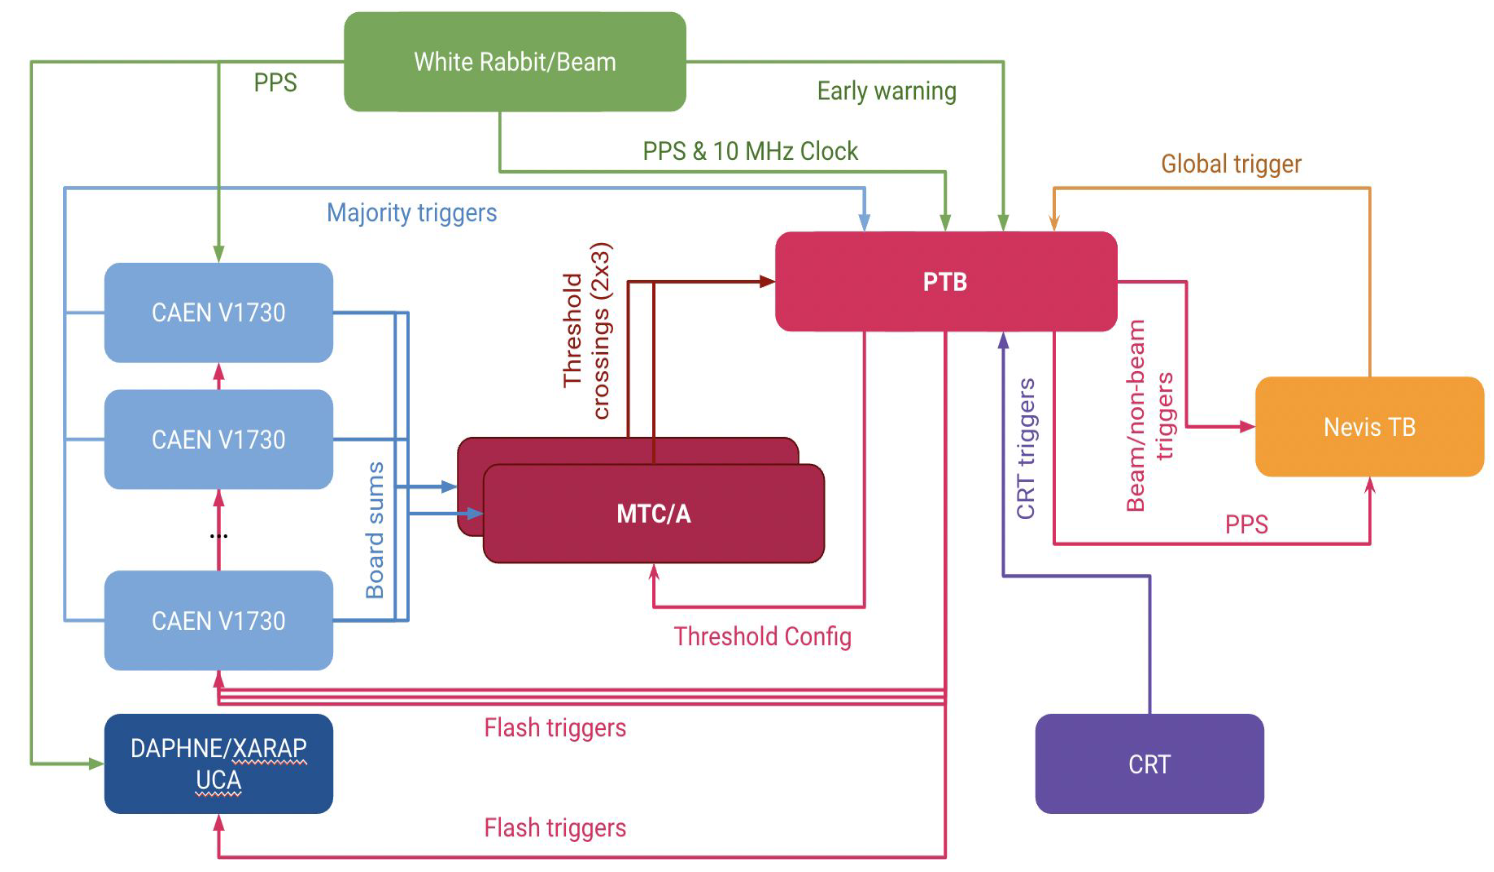
\includegraphics[width=0.95\textwidth]{SBND_Trigger}
\caption[SBND_PDS]{
Diagram displaying the flow chart of signals for the hardware triggering system at SBND.
Fig. from \cite{}.
}
\label{fig:SBND_Trigger}
\end{figure}
\subsection{Data Acquisition}

%\section{Overview of the Data Acquisition System}
\label{sec4DAQOverview}

The Data Acquisition (DAQ) system at SBND is responsible for transporting data from subsystem readouts to event builder machines. 
During real-time data flow, the DAQ has the capability to assemble data from each subsystem into a physics event, known as for event building. 
Additionally, the DAQ must be able to apply software metrics to filter events for various data streams and data monitoring purposes.
The DAQ acquires data from six subsystems, as illustrated in Fig. \ref{fig:daqOverview}. 
Among these, four are detection subsystems: the TPC, PMTs, X-ARAPUCAs, and CRTs. 
Furthermore, the other two subsystems include the PTB from the hardware triggering system and the SPEC-TDC, a specialized timing mezzanine to be discussed in Section \ref{}.
%Each detection subsystem incorporates specialized hardware components for digitizing and reading out the physical signals. 
%The PTB, as a hardware board within the SBND trigger system, is responsible to provide triggering signals to each detection subsystem independently.
%The SPEC-TDC is a specialised timing mezzanine module designed specifically for timestamping purposes.
%Further details about its functionality are outlined in section \ref{subsec42TimeRef}.

\begin{figure}[htbp] 
\centering    
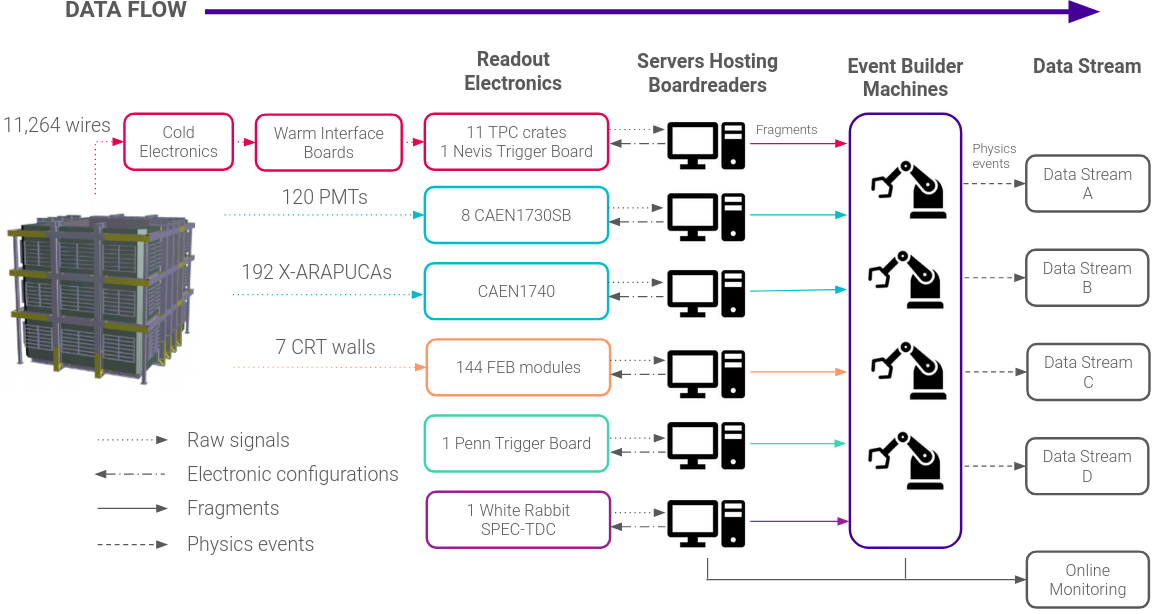
\includegraphics[width=0.90\textwidth]{DAQ_Overview}
\caption[DAQOverview]{
The DAQ system at SBND is responsible to acquire from 6 hardware readouts.
Each hardware component is accompanied by a corresponding software boardreader, serving as a communication bridge between the hardware and the event builder machines.
The event builders assemble physics events and send them to different data streams.
}
\label{fig:daqOverview}
\end{figure}

\subsubsection{TPC Readouts}
%TODO: ref Nevis ?

%Cold Electronic
The TPC readouts consist of two components: (1) the Cold Electronics (CE) readouts \cite{SBND_CE} and (2) the Nevis readouts. 
As depicted in Fig. \ref{fig:SBND_APA}, the wire planes are connected to CE readouts positioned at the top and on each side of the APAs.
Located inside the cryostat, the CE components are submerged in LAr to reduce thermal noise as well as cable lengths. 
They are responsible for amplifying and digitizing waveform signals at a sampling frequency of 2 MHz. 
Subsequently, the signals are sent outside of the cryostat to the Warm Interface Boards (WIBs) via copper cold cables. 
The WIBs serve as a bridge between the CE and other systems through fibre optic links.
This isolation architecture ensures the complete separation of wire grounding from the building, therefore resulting in a superior signal-to-noise ratio.

%Nevis Readout
Following the WIBs, the data is transmitted to the Nevis readouts, which are the subsequent warm electronics component in the TPC DAQ chain.
The Nevis readouts comprise 11 TPC crates responsible for reading out, buffering, and processing the wire signals. 
Additionally, the Nevis Trigger Board (NTB) provides two parallel independent streams of data.
The continuous stream requires no external triggers and outputs data with lossy compression. 
Meanwhile, the neutrino stream relies on the ETRIG signal from the PTB for triggering, and reads out data with lossless compression.

\subsubsection{PDS Readouts}

%CAEN digitizer
%X-ARAPUCA
The 120 PMTs are read out by 8 CAEN V1730SB digitizers \cite{caen1730}. 
This digitizer model is capable of recording waveforms for 16 channels independently, with a sampling rate of 500 MHz.
Meanwhile, the 192 X-ARAPUCAs are read out by 3 CAEN digitizers of a different model, VX1740B \cite{caen1740} \footnote{As of February 26, 2023: The readout design of X-ARAPUCAs is under development at the time of writing this thesis.}.
This digitizer model can readout 64 channels at a lower sampling frequency of 62.5 MHz. 
Both of these models feature deep buffers to store longer waveforms and handle higher data rates.
Notably, the V1730SB model offers better waveform baseline stability against temperature fluctuations. 
Multiple CAEN digitizers can be synchronised to form a complex system, such that they collectively behave as a single digitizer. 
The characterisation of synchronisation across multiple V1730SB digitizers is detailed in Section \ref{}.
%Thus, the following section evaluates the timing precision of CAEN digitizer by characterising the synchronisation across multiple digitizers.

\subsubsection{CRT Readouts}
%The timing resolution of the CRT readout electronics is evaluated in the following section.
%CRT FEB
The 7 CRT planes are read out by 144 Front End Board (FEB) modules \cite{crt_note}. 
Each FEB module is a multifunctional board capable of reading out 32 channels, with one channel per SiPM. 
The module can provide a bias voltage, which is adjustable for individual SiPM, as well as signal amplification and shaping.
Once the signal is shaped, the FEB can apply signal discrimination and self-triggering, such as coincidence for each pair of SiPMs in a CRT strip or coincidence across multiple FEBs for orthogonal CRT strips. 
Once the signal passes the trigger, it is digitised and timestamped with respect to an input reference clock. 
The data is then stored in a buffer and read out via an Ethernet connection. 
The characterisation of the timing resolution of FEB modules is detailed in Section \ref{}.
%The following section focuses on the characterisation on the timing resolution of the FEB module.

\subsubsection{Event Building}

The DAQ software framework is provided by the \textit{artdaq Toolkit}, developed by the Real-Time Systems Engineering Department of Fermilab's Scientific Computing Division \cite{artdaq_note}. 
This software serves as the backbone for communication between the hardware components and the event builder machines.
Within the \textit{artdaq} framework, each discrete hardware readout component has a corresponding software module known as a boardreader. 
These boardreaders facilitate communication between the readout electronics and the event builder machines. 
They can send configurations directly to the hardware in one direction and retrieve data from the hardware in the opposite direction, as illustrated by the arrow directions to and from the boardreaders in Fig. \ref{fig:daqOverview}.
%The following section provides an overview of the DAQ workflow at SBND as illustrated in Fig. \ref{fig:daqOverview}, describing how signals are acquired from the detection hardware and subsequently digitized by boardreaders and assembled into a physics event.
%describe boardreader fragment

The data is packaged into a digitized format called a fragment, as depicted in Fig. \ref{fig:fragmentDiagram}. 
The fragment class consists of a header containing experiment-specific information essential for event building, an optional metadata, and a data payload storing the hardware-defined data.
A fragment is generated by the boardreader when its corresponding hardware readout receives a trigger. 
The timestamp of the trigger arrival is encoded in the fragment header, known as the fragment timestamp. 
This timestamp is a crucial value in the event building process.

\begin{figure}[tbp!] 
\centering    
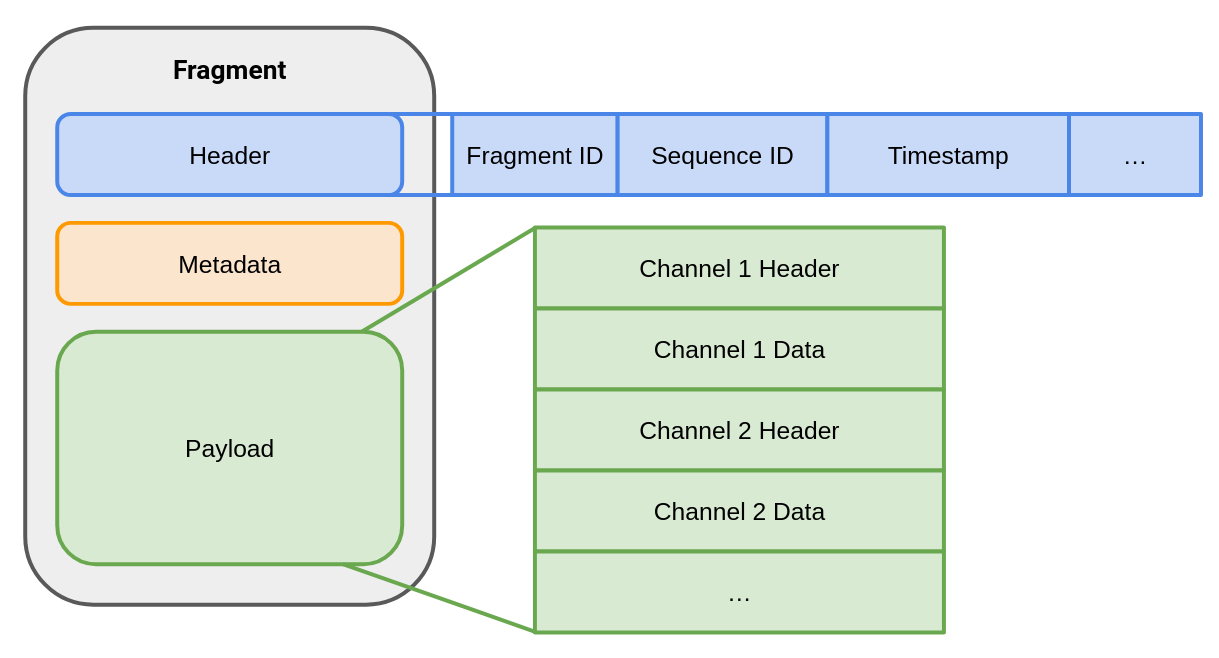
\includegraphics[width=0.6\textwidth]{Fragment_Diagram}
\caption[FragmentDiagram]{
Diagram illustrating the fragment class defined by the \textit{artdaq Toolkit}. 
The header contains the crucial fragment timestamp information needed for event building.  
%Optionally, the metadata structure contains hardware configurations. 
%The payload is designated for storing data from the hardware readout, of which the data structure is pre-defined by the hardware. 
}
\label{fig:fragmentDiagram}
\end{figure}

%what is push/pull

Once fragments are generated, boardreaders can send them to the event builders in one of two configurations: (1) push or (2) pull.
In the push configuration, the boardreader actively sends fragments continuously at the rate at which the fragments are generated. 
With each fragment sent, the push boardreader also creates a request message, which is multicast to all other boardreaders currently in pull mode. 
This request message contains the timestamp of the push fragment.
%The sequence ID of the fragments determines the sequence ID of the built event, ensuring  that every fragment is built as a single event.

In contrast to the push configuration, the boardreader in the pull configuration stores the fragments in its buffer as they are being generated. 
These fragments are sent to the event builders only upon receiving a request message.
The pull boardreader checks its buffer and selects the fragments with timestamps falling within a specified time window of the request message, known as a \textit{pull window}.
It then dispatches these selected fragments to the event builders. 
Subsequently, the event builder machines assemble this set of pull fragments, together with the one push fragment that initially generated the request message, into a single event.
%To determine which fragments to send, the boardreader has a configurable parameter called pull window, which specifies a time window relative to the timestamp of the request message.
%The pull boardreader checks its buffer and selects the fragments with timestamps falling within this defined time window.
%The selected fragments that meet the timestamp requirement are then dispatched to the event builders.
%The sequence ID of the resulting event is determined by the push fragment.

\begin{figure}[htbp!] 
\centering    
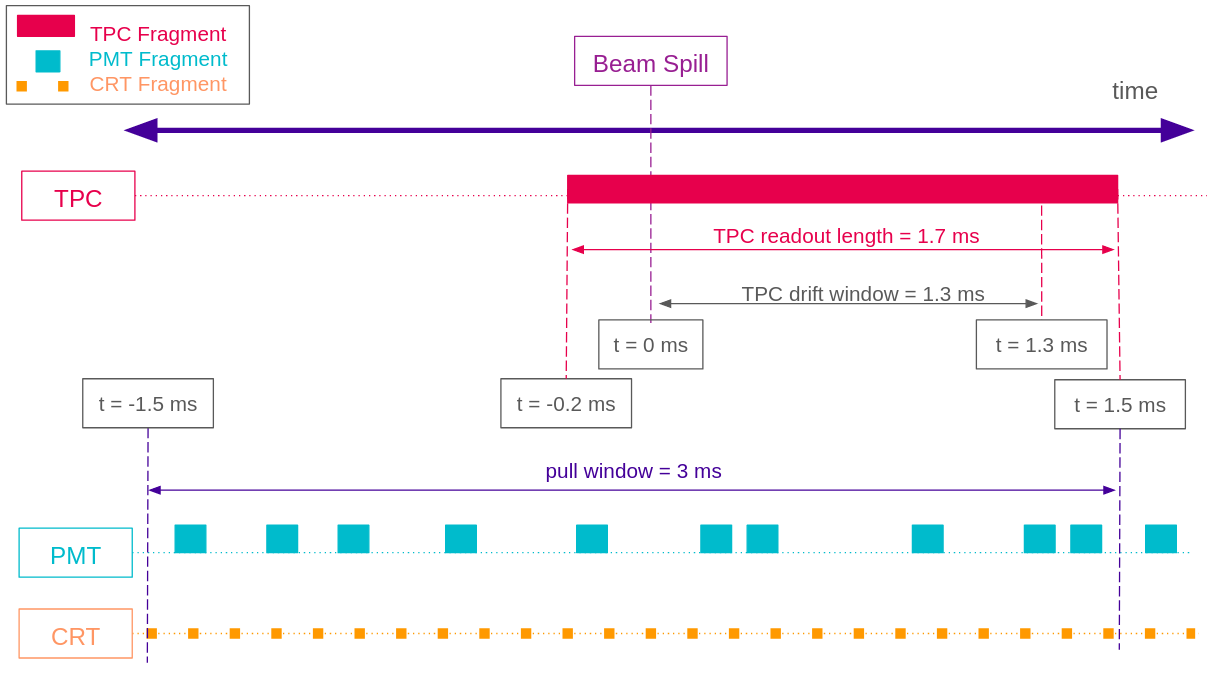
\includegraphics[width=0.75\textwidth]{SBND_Event_Structure}
\caption[SBNDEventStructure]{
Diagram depicting structure of a neutrino beam event at SBND, where the time axis is centred at 0 for when the beam spill begins. 
The event contains TPC fragments of readout length 1.7 ms to fully cover the drift window of ionised electrons. 
The PMT and CRT fragments are included 1.5 ms before and after the beam spill starts. 
The time asymmetry of the event structure is due to scintillation photon signals propagating faster compared to electron signals.}
\label{fig:SBNDEventStructure}
\end{figure}

%describe an event structure
A neutrino beam event at SBND is structured as outlined in Fig. \ref{fig:SBNDEventStructure}, with examples provided for TPC, PMTs, and CRTs fragments.
The PTB first sends a single ETRIG to the NTB that coincides with the start of the BNB beam spill if it determines a neutrino event occurs. 
This generates a TPC fragment with a readout length of 1.7 ms, covering the entire TPC drift length of 1.3 ms and including a padding of 0.2 ms before and after the drift. 
The ETRIG timestamp is encoded in the NTB fragment header.
The NTB boardreader operates in push configuration, thus driving the data acquisitions of the PMT and CRT readouts in pull configuration.
%Within this structure, there is only one push boardreader that increments the event sequence ID counter whilst the remaining boardreaders run in pull configuration.
%The push boardreader is called the Nevis Trigger Board (NTB), which is a component of the hardware complex to readout the TPC data. 

%Meanwhile, the boardreaders for the PMTs and CRTs are in pull mode.
The PTB sends multiple FTRIGs to the PMT readouts throughout the beam spill, while the CRT readouts are self-triggered independently. 
The fragment readout lengths from the PMTs and CRTs readouts are much shorter compared to TPC fragments, on the order of $\mu$s and ns, respectively.
The pull window is defined to be 3 ms centred on the timestamp of the NTB fragment. 
This window includes PMT and CRT fragments generated 1.5 ms before and after the beam spill starts. 
Subsequently, the event builders package all these fragments together to form a physics event.

%event asymmetry
The event structure has an asymmetry in time due to the different physics characteristics of photon signals, detected by the CRTs and PMTs, and electron signals, detected by the TPC wires. 
Photon signals propagate much faster than electron signals.
Specifically, a photon produced in a CRT scintillator strip takes approximately 5 ns to travel from the far end of the strip until reaching a SiPM. 
Similarly, a photon produced in the TPC takes a maximum of 15 ns to arrive at the PMTs from the scintillation location.
In contrast, an ionised electron produced at the same time in the TPC takes 1.3 ms to fully drift from the cathode to the anode. 
Consequently, scintillation photon signals produced during the beam spill need to be digitized and read out much earlier compared to the electron signals.

\subsubsection{Data Stream}

%describe a data stream
After the event builder machines complete building a physics event, the resulting event can be filtered and sent to various storage locations for different analysis purposes, commonly referred to as data streaming.
The \textit{artdaq Toolkit} provides options to incorporate customisable filtering steps in real-time. 
This allows the event builders to apply complex software metrics based on the fragment contents of an event. 
Once an event successfully passes through the filter, the event builders send it to a location defined by the filter for storage, as illustrated by the arrow directions from the event builders in Fig. \ref{fig:daqOverview}. 
However, if an event fails to pass the filters, it will be dropped in real-time.

%data monitoring?
The \textit{artdaq Toolkit} also includes a built-in process for streaming data between event builder machines and online monitoring platforms.
While operating in real-time, fragments from boardreaders and physics events can be transmitted to these platforms for various monitoring purposes. 
SBND currently employs two online platforms to monitor the health of the DAQ: (1) Grafana and (2) Minargon.

Grafana provides real-time monitoring of the status of processes being run by boardreaders and event builders, as well as some status of the respective hardware components for each boardreader. 
An example of Grafana website is displayed in Fig. \ref{fig:Grafana} for the boardreaders of PMTs.
In the top left panel, the run number and a dial indicating the trigger rate issued by the PTB at 5.60 Hz are shown. 
The right panels display 9 dials, corresponding to 9 CAEN digitizers, showing the PMT fragment rates sent by the digitizers in good agreement with the trigger rate.
The bottom left graph illustrates the PMT fragment rates as a function of time. 
The bottom middle and right graphs depict the rates of empty and missing PMT fragments as a function of time, which remain flat at zero, indicating a healthy state.

\begin{figure}[htbp!] 
\centering    
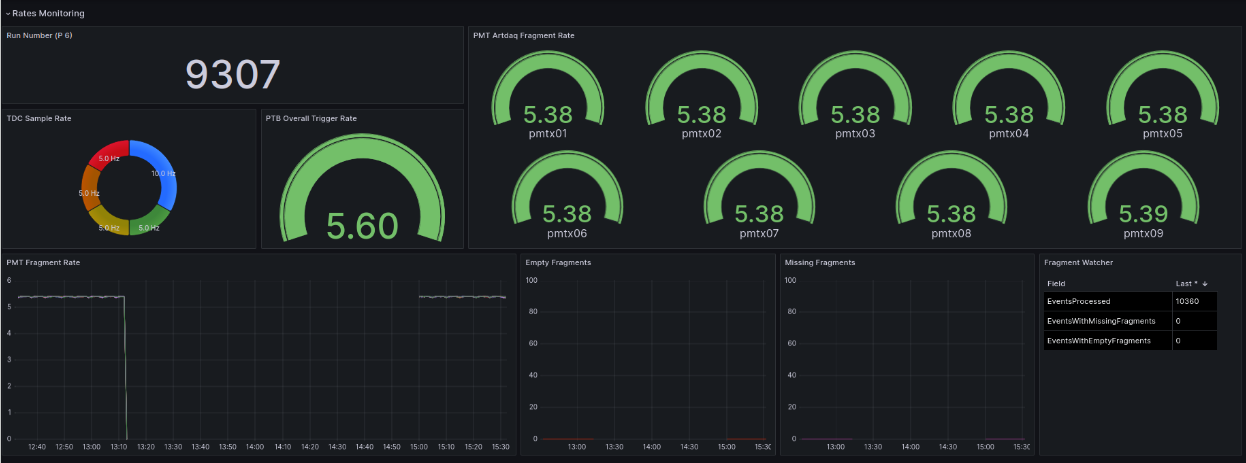
\includegraphics[width=1.0\textwidth]{Grafana}
\caption[Grafana]{
Screenshot displaying a section of the Grafana monitoring website for the boardreaders of the PMT readouts.
The green large dial in the left panel shows the trigger rate from the PTB at 5.60 Hz, while the 9 smaller green dial in the right panel shows the fragment rates from PMT boardreaders in good agreement with the trigger rate.
}
\label{fig:Grafana}
\end{figure}

Moreover, Minargon provides real-time data quality monitoring. 
This online monitoring process applies simple reconstruction and event display to quantitatively verify the physics characteristics of an event. 
An example metric is displayed in Fig. \ref{fig:Minargon}, which shows the root mean square of the PMT waveform baselines as a histogram in the left plot and as a function of time in the right plot.
This metric helps monitoring the baseline equalisation and stability over time.
%The author has worked extensively on developing the monitoring processes for the DAQ of the PMTs on both Grafana and Minargon monitoring platforms during her PhD course. 

\begin{figure}[htbp!] 
\centering    
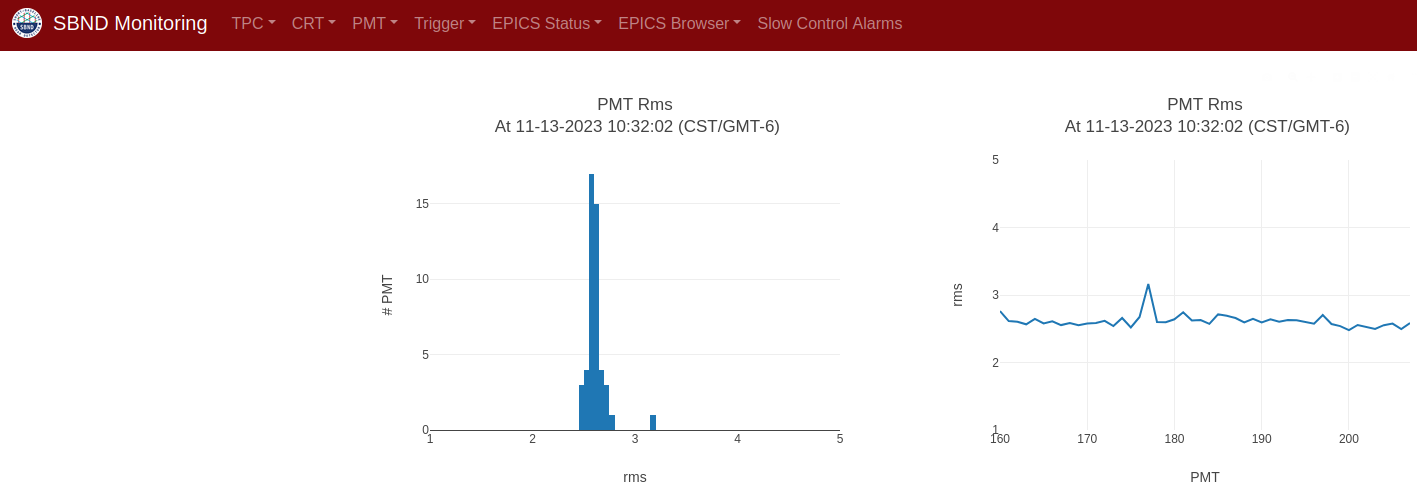
\includegraphics[width=1.0\textwidth]{Minargon}
\caption[Minargon]{
Screenshot displaying a section of the Minargon website to monitor quality of data acquired by the PMT DAQ.
The metric shown here is the waveform baseline RMS, plotted as a histogram (left) and as a function of time (right).
}
\label{fig:Minargon}
\end{figure}

%********************************** %First Section  **************************************
\section{The Booster Neutrino Beam}
\label{sec4BNB}

%Describe rate
The SBND detector directly measures the neutrino flux coming from the BNB. 
A comprehensive technical details of the BNB can be found in Ref. \cite{BNBMiniBooNE}.
The BNB operates by extracting protons with a kinetic energy of 8 GeV from the Booster synchrotron in spills made up of 7 to 11 pulses in a row at a frequency of 15 Hz, averaging to a rate of $\sim$5 Hz.
Each spill delivers $5 \times 10^{12}$ protons within a beam spill window lasting 1.6 $\mu$s.
The structure of a beam spill structure consists of 81 individual neutrino bucket, with a Gaussian width of 1.308 ns and a spacing of 19 ns \cite{BNBsigma}.
This distinctive bucket structure can be resolved with sufficient timing resolution, enabling cosmics rejection and BSM physics searches occurring outside of the bucket.
Fig. \ref{fig:CRT2017} illustrates such capability of the Cosmic Ray Tagger (CRT) system at SBND, which collected data from the BNB from 2017 to 2018 \cite{CPAD2022}.

\begin{figure}[htbp] 
\centering    
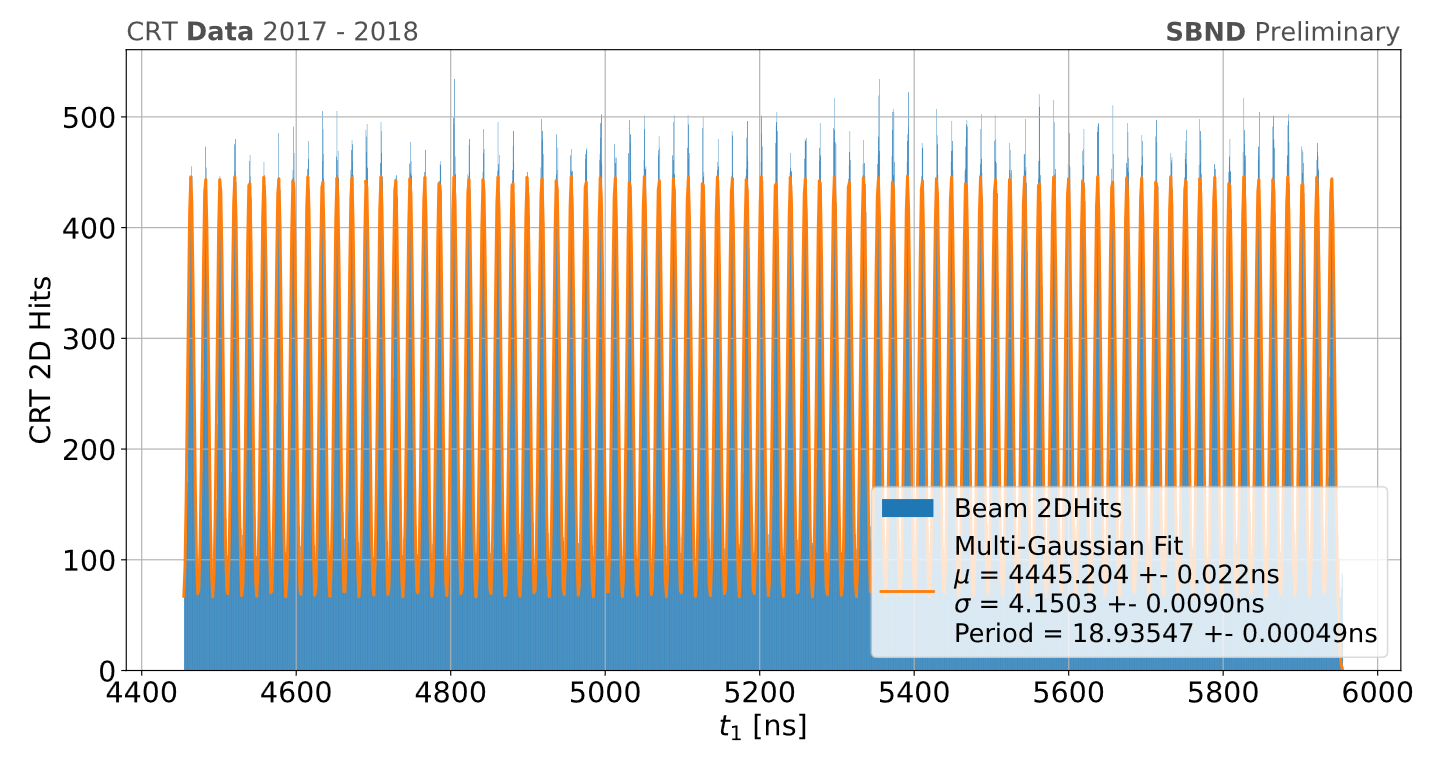
\includegraphics[width=0.75\textwidth]{CRT2017}
\caption[CRT2017]{
The BNB beam structure was measured and resolved using the CRT system of SBND as a beam telescope during a run from 2017 - 2018.
The beam structure can be seen, made up of 81 neutrino buckets.
Fig. from \cite{CPAD2022}.
}
\label{fig:CRT2017}
\end{figure}

%hardware structure
The neutrino production process in the BNB is illustrated in Fig. \ref{fig:BNBDiagram}.
Initially, protons are injected into the Booster synchrotron and accelerated from 400 MeV to 8 GeV kinetic energy. 
Their intensity is measured by two steroids, while their positioning and timing are monitored by beam position monitors and Resistive Wall Monitor (RWM) \cite{BNBRWM}.
Upon exiting the Booster, the proton beam traverses focusing and defocusing quadrupole and dipole magnets before being steered and focused onto the target of the BNB.
The target consists of a beryllium cylinder measuring 71.1 cm in length and 0.51 cm in radius.
The choice of beryllium was motivated by its replaceable ability in the event of radioactivity issues, as well as its ability to facilitate sufficient energy loss via an air cooling system.
The target is placed inside a pulsed horn system, which acts as a 170 kA electromagnet to focus the secondary mesons resulting from protons colliding on the target.
The polarity of the horn can be adjusted to focus positive (negative) mesons for operation in neutrino (antineutrino) mode. 
Downstream of the horn assembly, a concrete collimator of dimensions 214 cm in length and 30 cm in radius (expanding to 35.5 cm from upstream to downstream end) absorbs particles that do not contribute to the neutrino flux, thereby reducing radiation elsewhere in the beamline.
The focused particles then propagate through an air-filled cylindrical decay region spanning 45 m, terminated by a steel and concrete absorber located 50 m from the upstream face of the target.
Secondary mesons decay into tertiary neutrinos within this region, while long-lived muons are absorbed by the absorber. 
Subsequently, the neutrinos traverse through a dirt region before reaching the SBND detector.

\begin{figure}[tbp] 
\centering    
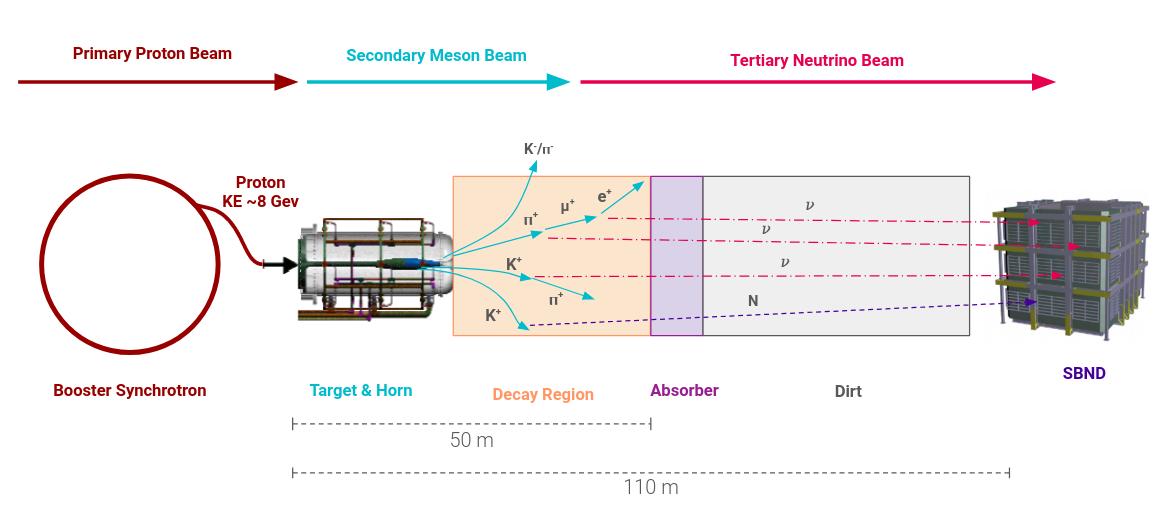
\includegraphics[width=1.0\textwidth]{BNBDiagram}
\caption[BNBDiagram]{
Diagram of the neutrino production in the BNB.
Primary proton beam (brown arrow) is collided onto the target to produce secondary mesons (blue arrows), which subsequently decay into tertiary neutrinos (pink arrows).
The production mode for heavy neutral leptons from kaon decays is also shown (purple arrow).
}
\label{fig:BNBDiagram}
\end{figure}


%beam simulation
%Explain what meson is in the flux, what tuning is used, 
The beam is simulated using GEANT4 with different tunings for the composition of the secondary mesons and hadrons produced from $p + Be$ interactions \cite{BNBMiniBooNE}.
The $\pi^{\pm}$ production is tuned to the HARP data set using Sanford-Wang parametrisation .
The $K^{+}$ production is extrapolated to the global $K^{+}$ production data using Feynman scaling-based parametrisation, and further constrained by SciBooNE's direct measurements of $K^{+}$ production from the BNB \cite{SciBooNE}. 
Other secondary hadrons and mesons such as $p$, $n$ and $K^{-}$ are modelled using the MARS hadronic interactions, however their overall contribution to the neutrino flux is small. 
Interaction cross sections of $p/n + Be$ and $\pi^{\pm} + Be$ are also incorporated in flux predictions \cite{DavePhd}.   
The systematics uncertainties associated the BNB flux are calculated by a re-weighting process, which will be presented in Chapter \ref{}.

Fig. \ref{fig:BNB_Meson_Flux} depicts the primary contributors to the secondary meson fluxes at the BNB, namely pions and kaons.
A small fraction of muons resulting from pion decays also contribute to the fluxes.
These fluxes are shown for the BNB operating in neutrino mode, mainly composed of positively charged mesons.
As discussed in Sec. \ref{sec2Production}, the flux of HNL comes from $K^{+}$ decays, which has energy peaking at $0.5 \sim 1$ GeV.
Ref \cite{BNBMiniBooNE} has highlighted significant uncertainties in the $K^{+}$ production cross sections within this energy range.
However, results from the SciBooNE experiment have demonstrated the validity of extrapolating higher energy $K^{+}$ data to the 1 GeV region using Feynman scaling \cite{SciBooNE}. 

\begin{figure}[bhtp]
\begin{subfigure}{.5\linewidth}
\centering
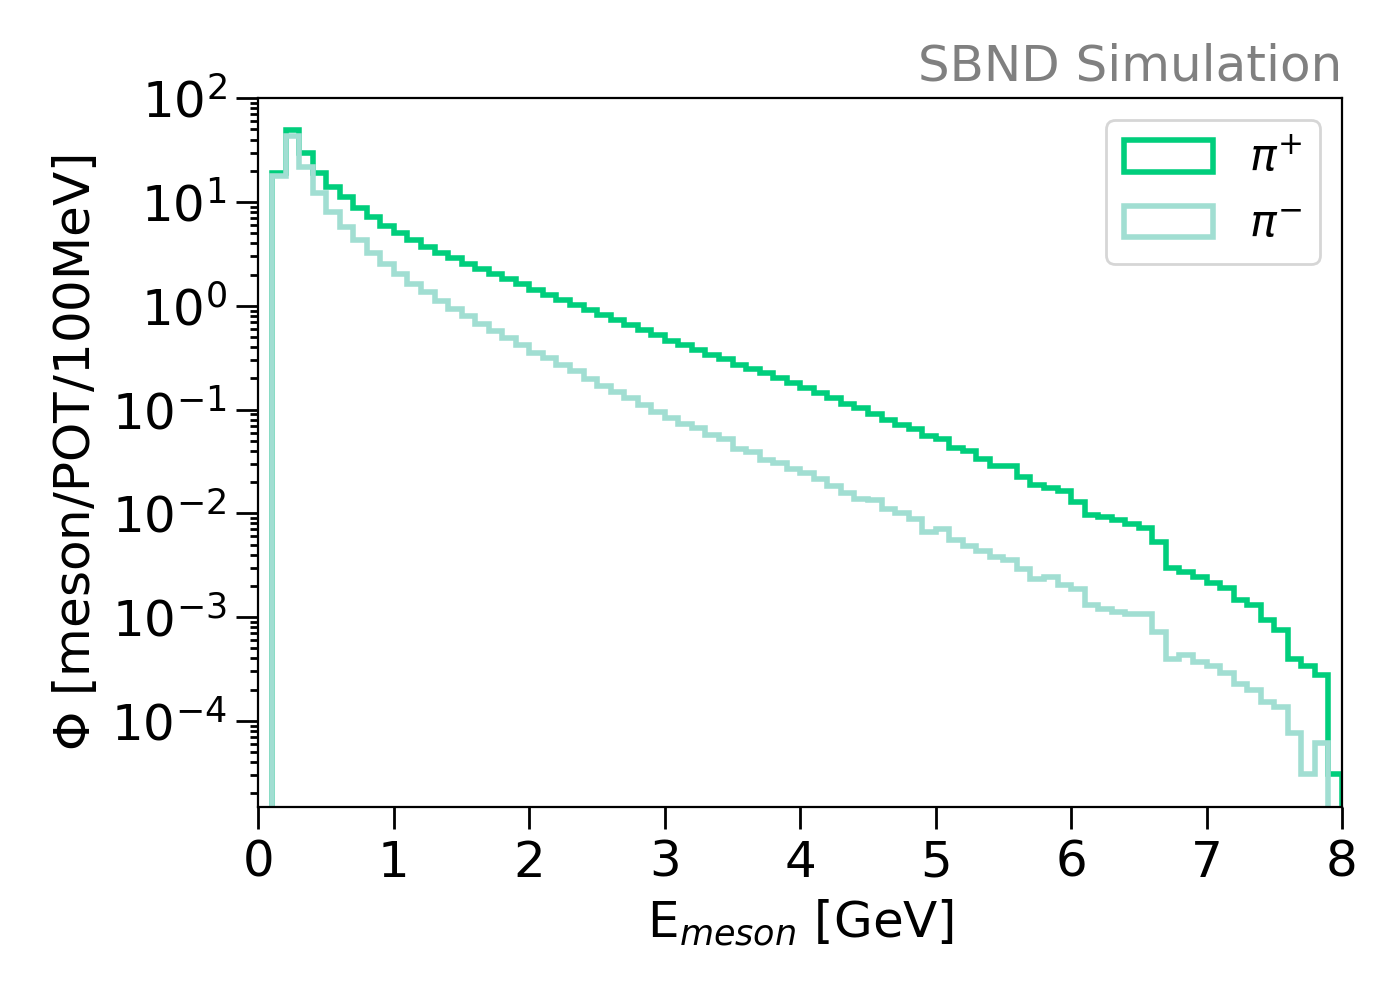
\includegraphics[width=0.90\textwidth]{BNB_Meson_Pion_Flux}
%\caption{}
%\label{fig:sub1}
\end{subfigure}%
\begin{subfigure}{.5\linewidth}
\centering
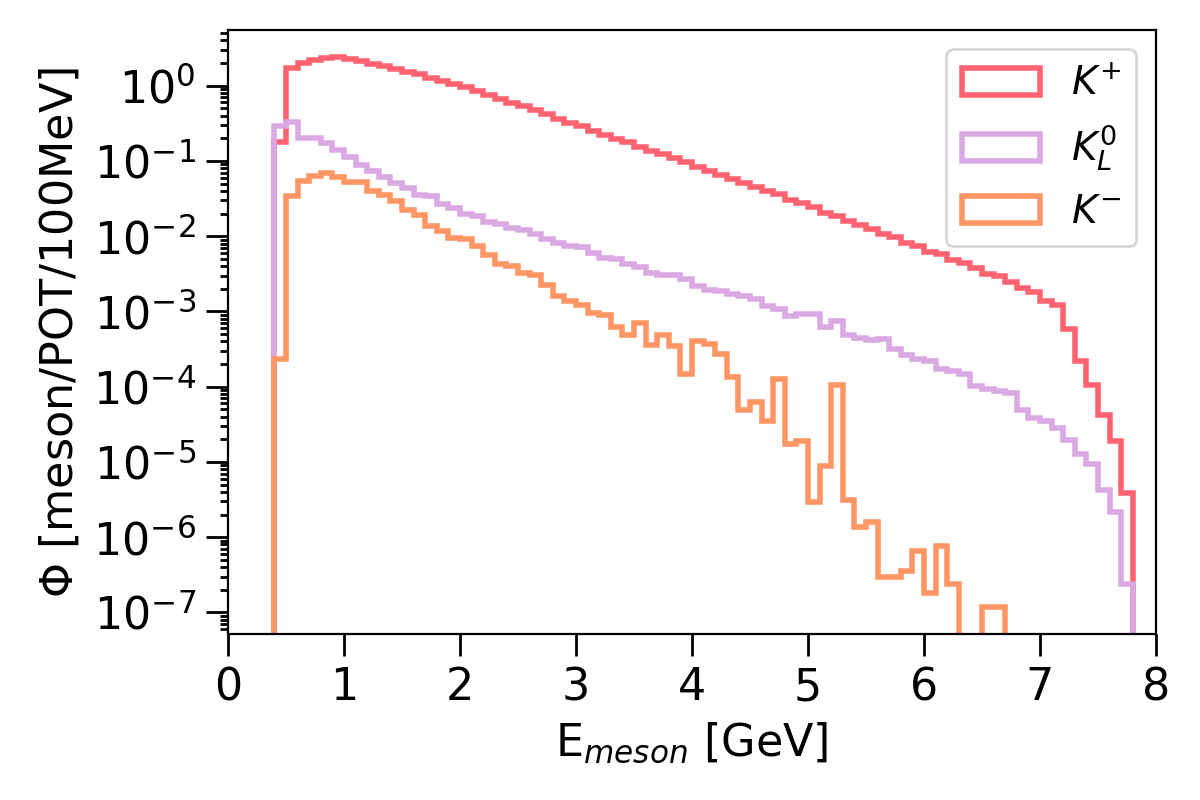
\includegraphics[width=0.90\textwidth]{BNB_Meson_Kaon_Flux}
%\caption{}
%\label{fig:sub2}
\end{subfigure}\\[1ex]
\begin{subfigure}{\linewidth}
\centering
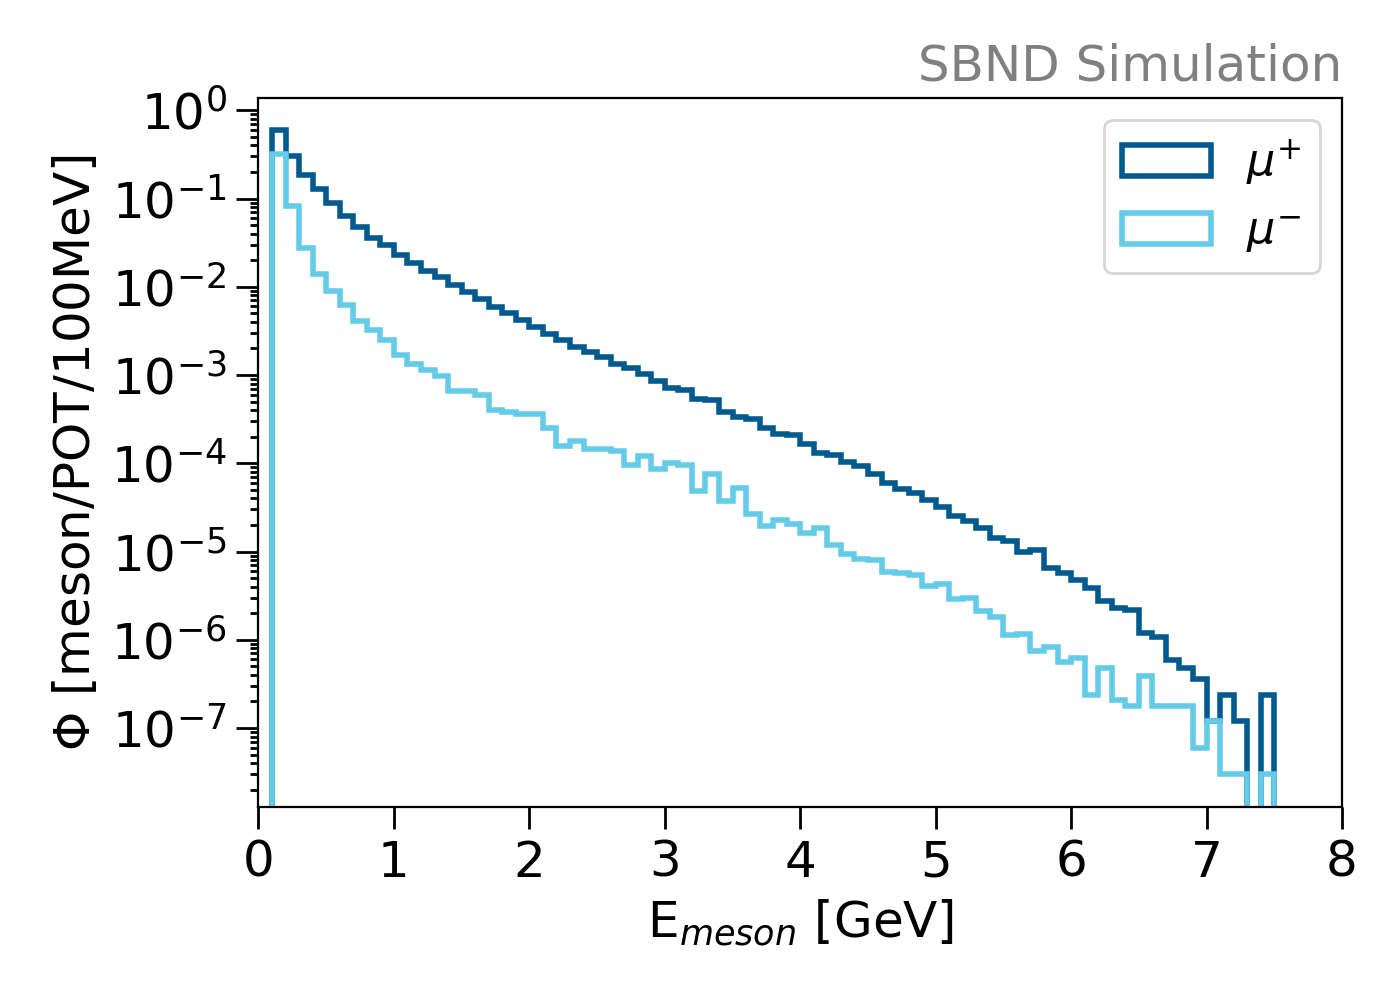
\includegraphics[width=0.45\textwidth]{BNB_Meson_Muon_Flux}
%\caption{}
%\label{fig:sub3}
\end{subfigure}
\caption{
Simulated fluxes of three main contributors to the secondary mesons produced in the BNB as a function of their energies: pions, kaons and muons. 
}
\label{fig:BNB_Meson_Flux}
\end{figure}
The simulation of the neutrino flux at the front face of SBND is depicted in Fig. \ref{fig:BNB_combined_neutrino_flux}, shown for different flavours of neutrinos. 
The flux is predominantly composed of $\nu_{\mu}$ ($\sim90\%$), followed by $\bar{\nu}_{\mu}$ ($\sim9\%$), while the combination of $\nu_{e}$ and $\bar{\nu}_{e}$ contributes less than 1\%.
Fig. \ref{fig:BNB_neutrino_flux} depicts the parent mesons for each neutrino flavour.
Pion production the dominant mechanism for both $\nu_{\mu}$ and $\bar{\nu}_{\mu}$, followed by kaon and muon production. 
Notably, a peak in the $\nu_{\mu}$ flux can be seen at half the mass of the kaon (235.5 MeV) resulting from kaon decay at rest \cite{kaonDecayNu}.
In the case of $\nu_{e}$, muons produced from pion decay is the primary source at low energies, while kaon production becomes the dominant mode at higher energies. 
Finally, $\bar{\nu}_{e}$ mainly originates from $K^{0}_{L}$ production.

%TODO: Make plots font bigger
\begin{figure}[hp] 
\centering    
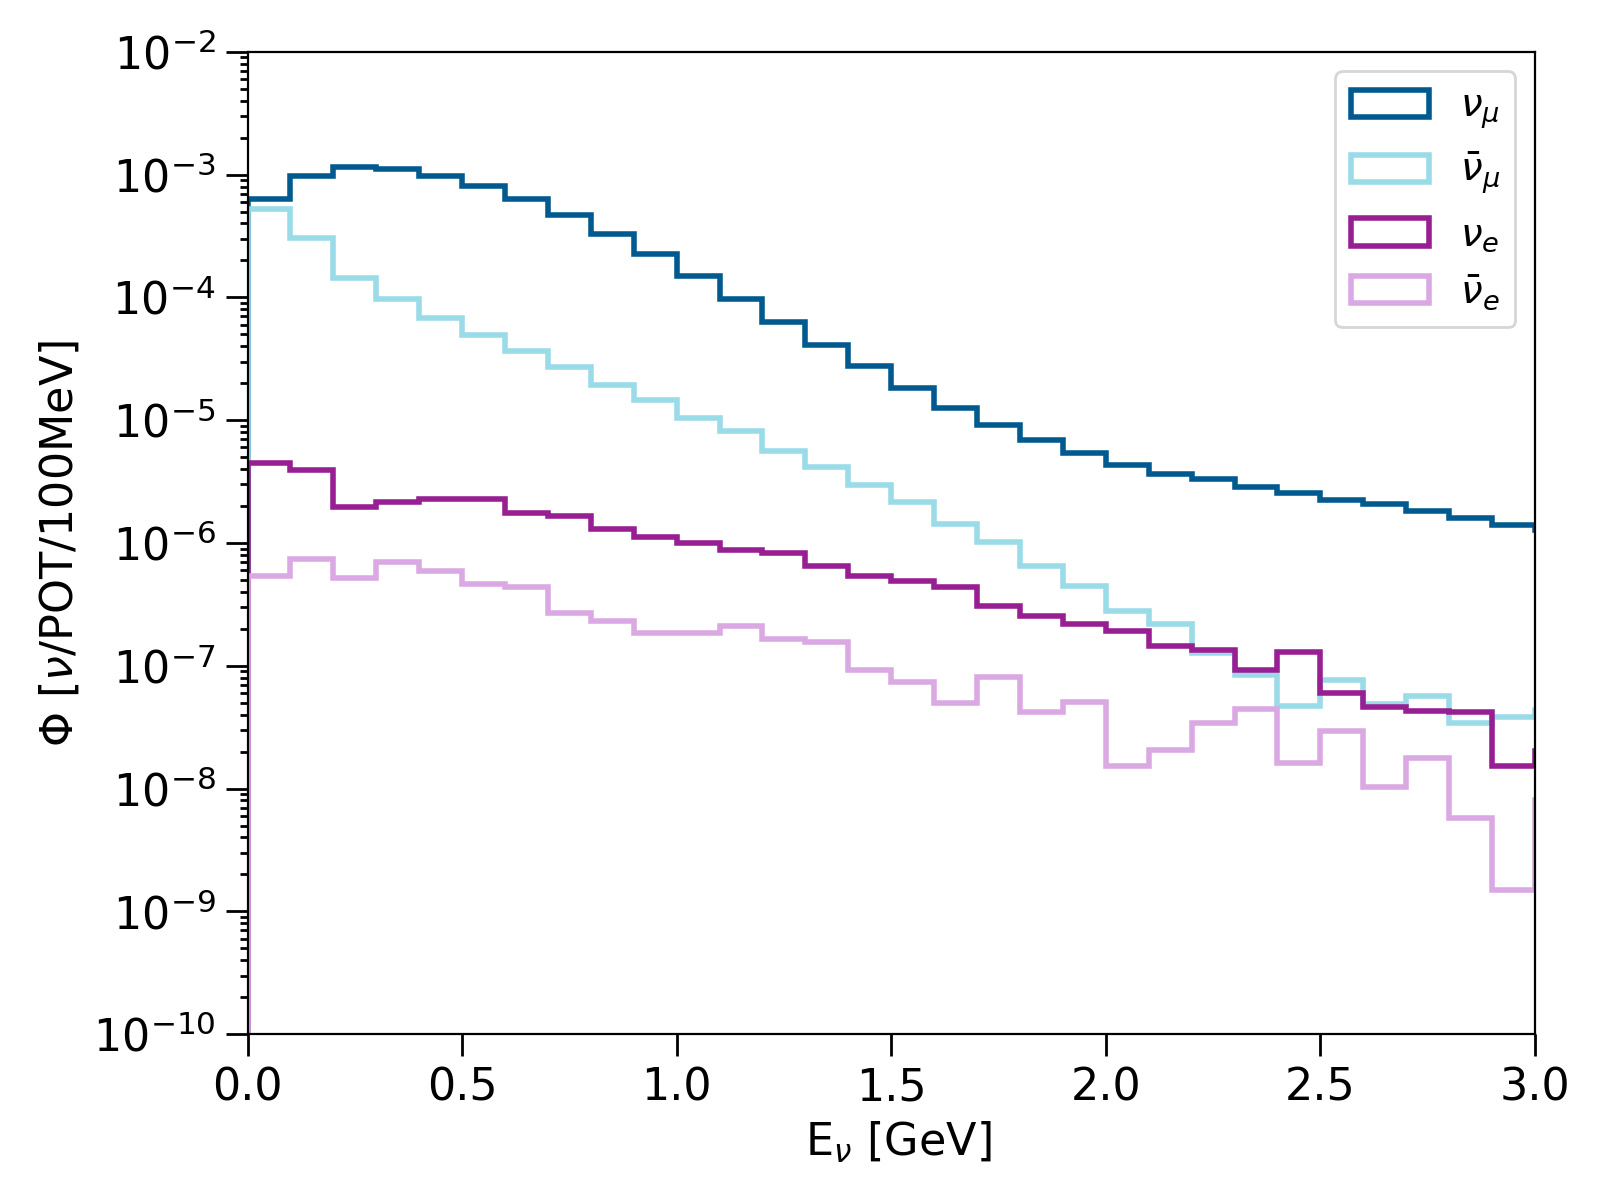
\includegraphics[width=0.45\textwidth]{BNB_combined_neutrino_flux}
\caption[BNB_combined_neutrino_flux]{
Simulated neutrino fluxes as a function of energy from the BNB at the front face of the SBND detector. 
}
\label{fig:BNB_combined_neutrino_flux}
%\end{figure}
%\begin{figure}[h] 
\centering    
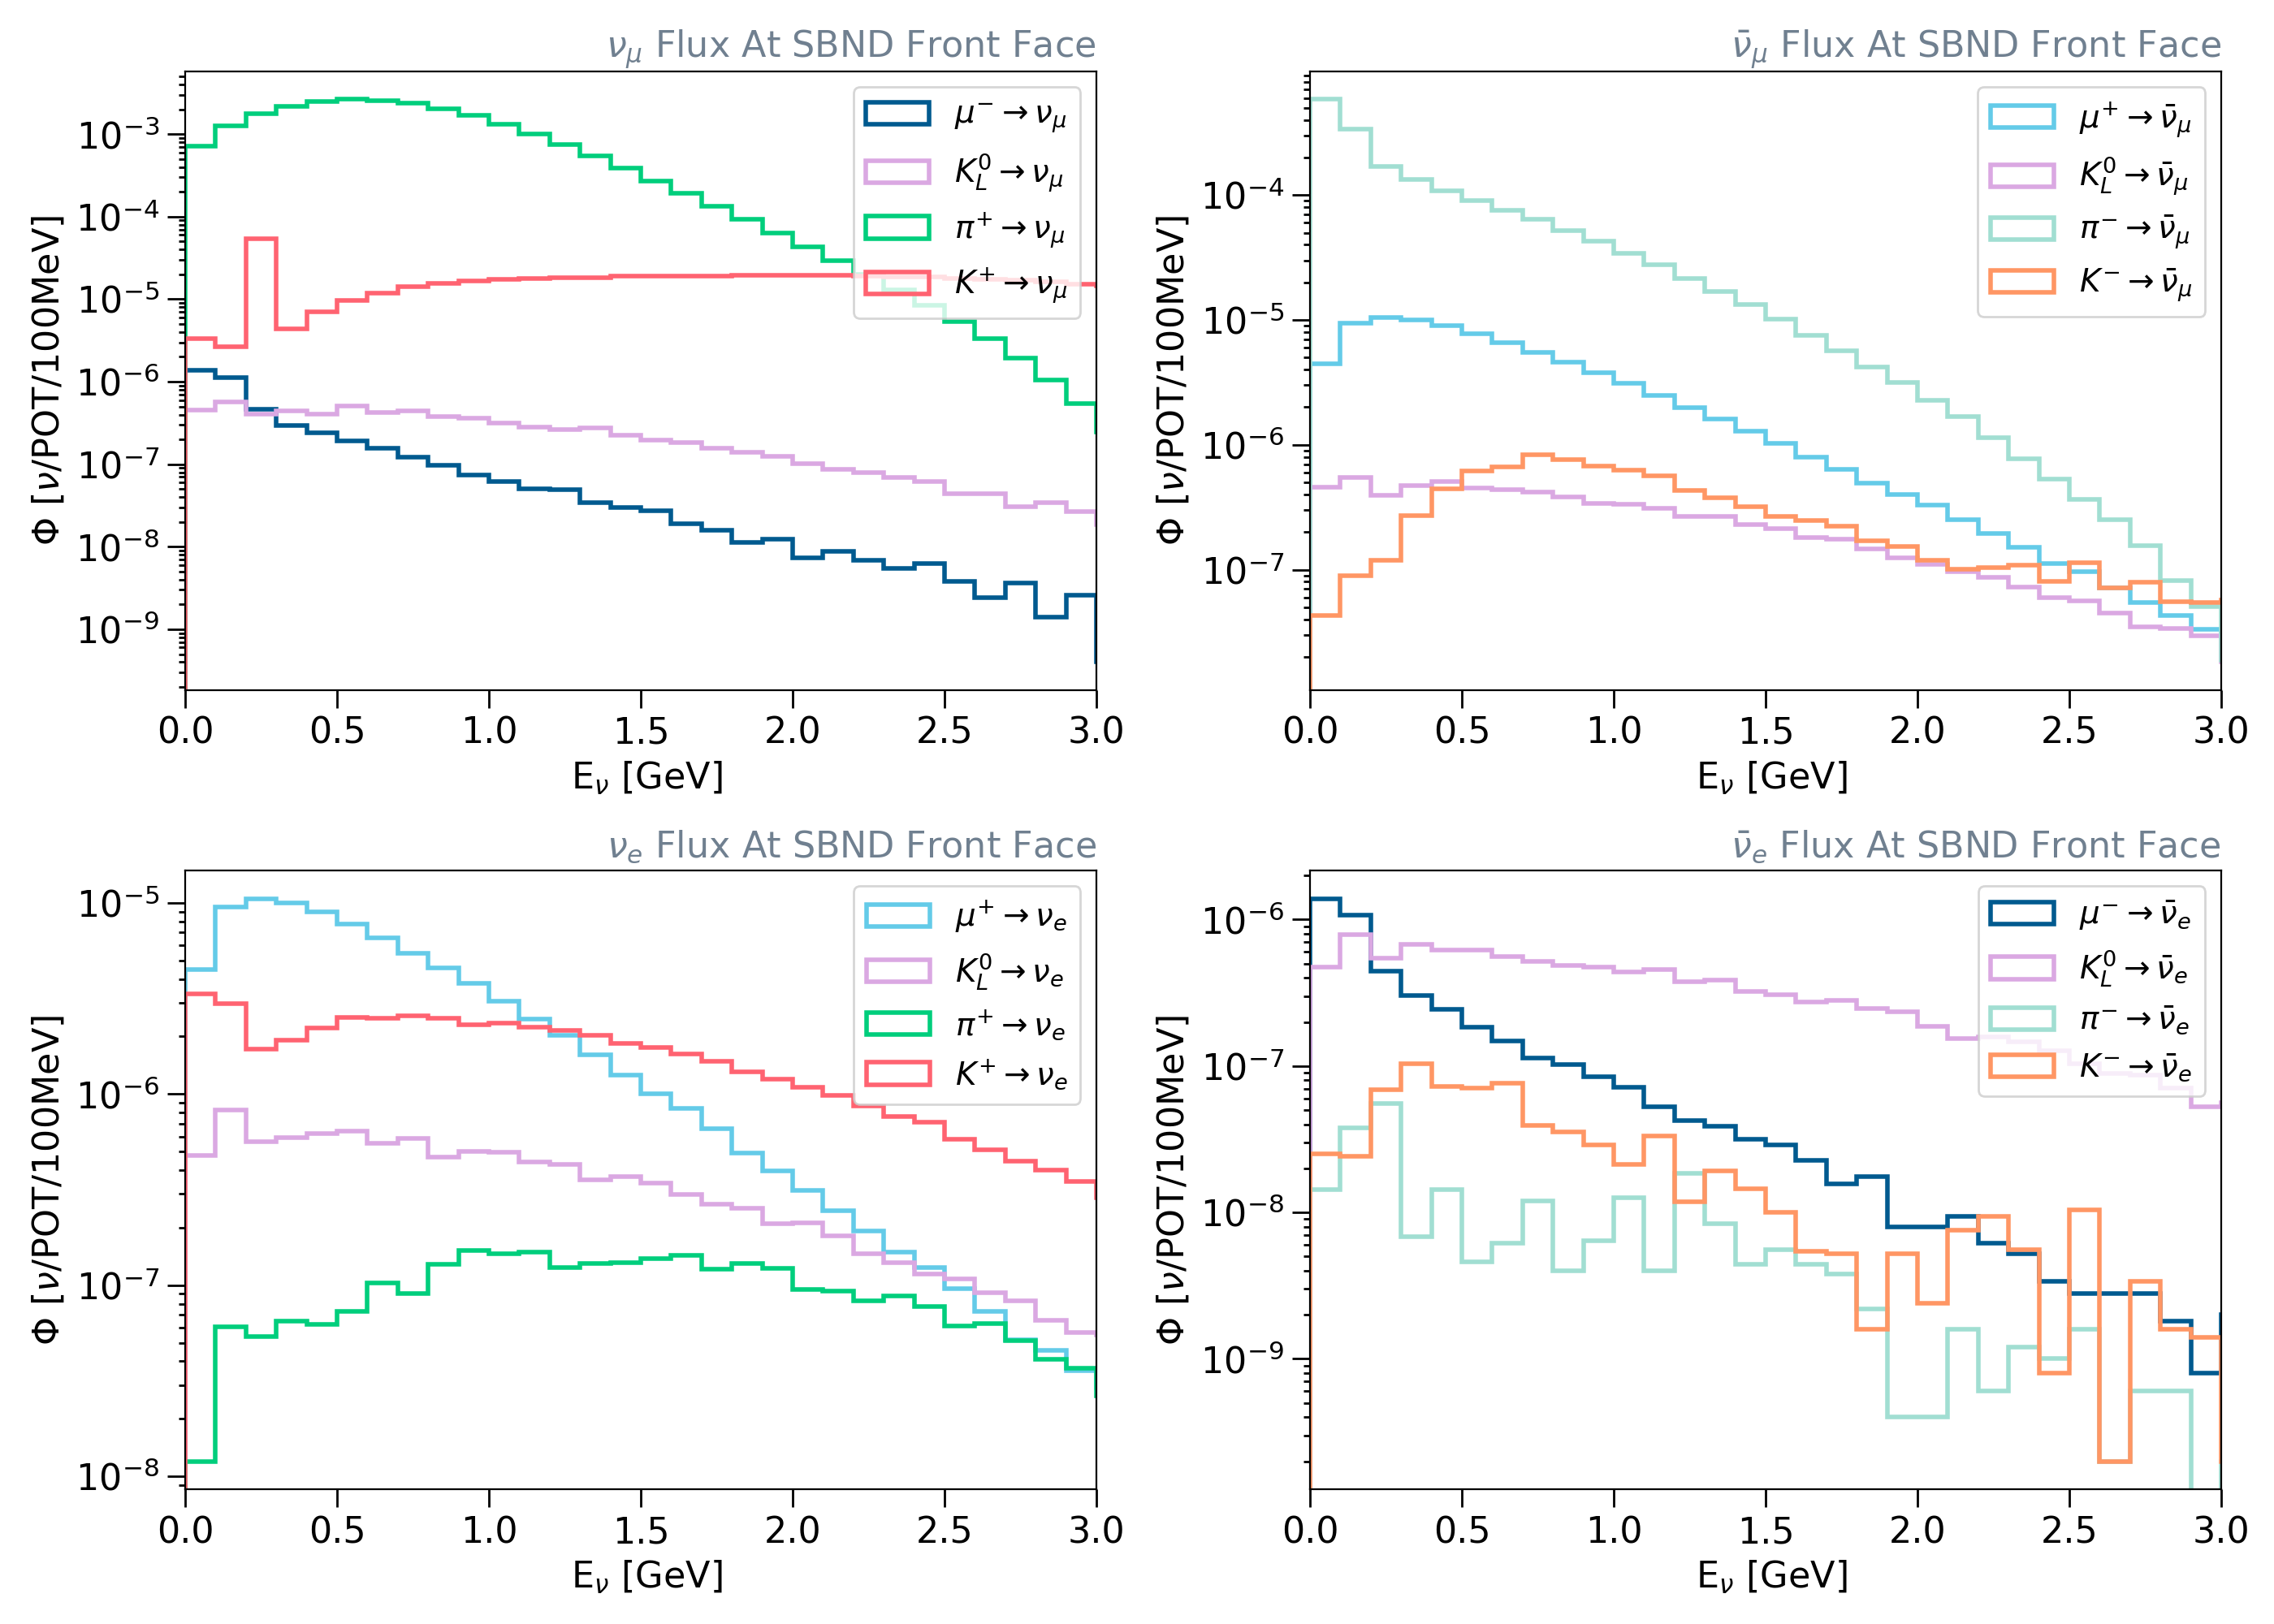
\includegraphics[width=0.81\textwidth]{BNB_neutrino_flux}
\caption[BNB_neutrino_flux]{
Simulated fluxes for different flavours of neutrino as a function of energy at the front face of SBND, broken down into types of parent mesons.
}
\label{fig:BNB_neutrino_flux}
\end{figure}
%********************************** %First Section  **************************************
\section{Concluding Remarks}

The SBND experiment, serving as the near detector of the SBN program, aims to conclusively address the low energy excess observed across experiments such as LSND, MiniBooNE, and others, including nuclear reactor and solar neutrino experiments. 
SBND will play a crucial role in constraining systematic uncertainties by measuring a large statistics of the unoscillated neutrino flux from the BNB.
Additionally, SBND has a rich physics program covering neutrino cross-section measurements and searches for BSM physics. 
Of particular relevance to this thesis, SBND aims to establish competitive limits on the sensitivity of HNLs within the probable mass range from the BNB.

The SBND detector measures the flux coming from the BNB, with the secondary $K^{+}$ meson being the primary contributor to the flux of HNLs.
The BNB has a distinctive bucket structure such that experiments with sufficient timing resolution can identify interactions occurring outside the neutrino buckets for cosmic rejection and BSM searches. 
Moreover, the hardware of SBND comprises three key detection subsystems: the TPC, the PDS, and the CRT system, alongside the hardware triggering subsystem. 
Each of these subsystems has dedicated readout electronics, which are managed by a complex data acquisition system.
The event building process of the DAQ relies on the timing information acquired from each subsystem. 
This process assembles the foundation of physics event upon which low-level and high-level reconstructions are built to achieve nanosecond timing resolution.
Therefore, the timing characterisation of the readout electronics will be discussed in the forthcoming chapter.
